\documentclass[10pt,a4paper]{article}
\usepackage[utf8]{inputenc}
\usepackage{amsmath}
\usepackage{amsfonts}
\usepackage{graphicx}
\usepackage{longtable}
\usepackage{todonotes}
\graphicspath{ {./images/} }
\usepackage{amssymb}
\usepackage[left=2cm,right=2cm,top=2cm,bottom=2cm]{geometry}
\usepackage{listings}
\usepackage{xcolor}
\usepackage{xparse}
\definecolor{codegreen}{rgb}{0,0.6,0}
\definecolor{codegray}{rgb}{0.5,0.5,0.5}
\definecolor{codepurple}{rgb}{0.58,0,0.82}
\definecolor{backcolour}{rgb}{0.97,0.95,0.92}



\lstdefinestyle{mystyle}{
    backgroundcolor=\color{backcolour},   
    commentstyle=\color{codegreen},
    keywordstyle=\color{magenta},
    numberstyle=\tiny\color{codegray},
    stringstyle=\color{codepurple},
    basicstyle=\ttfamily\footnotesize,
    breakatwhitespace=false,         
    breaklines=true,                 
    captionpos=b,                    
    keepspaces=true,                 
    numbers=left,                    
    numbersep=5pt,                  
    showspaces=false,                
    showstringspaces=false,
    showtabs=false,                  
    tabsize=2
}
\lstset{style=mystyle}
\newcommand{\te}{\texttt}
\usepackage[colorlinks = true,
            linkcolor = blue,
            urlcolor  = codegreen,
            citecolor = blue,
            anchorcolor = blue]{hyperref}
            \author{Zainab Nazari, and Carl Stermann-L\"ucke}
\title{Python Note}
\date{}



%%%%%%%%%%%%%%%%%%%%%%%%


\begin{document}




\maketitle
\tableofcontents












\section{Installation, read, write, and run}
If you own a Google account you do not need to install anything! Because you can use colaboratory of google. This is the easiest that you can reach to a python notebook and run your code.
In the   \href{https://colab.research.google.com}{colaboratory website}  you can read and write and run the python codes.
We generally need to tell apart two different ways of running python
\begin{itemize}
\item \textbf{Interactive Python}, by using the terminal you can interactively write and run a python code line by line. You just need to call python, and use it interactively in your terminal. For example
\begin{figure}[h]\centering
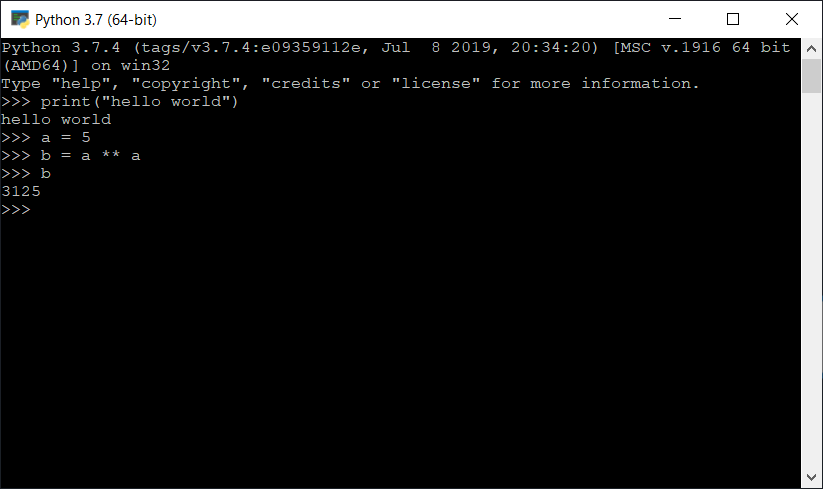
\includegraphics[width=0.7\textwidth]{interactive-python-terminal.PNG}
\end{figure}
\item \textbf{Python Scripts} (.py), which can be written in any editor and run in the terminal. To run a python code, we need to go to the folder/directory where the code is saved, then type \texttt{\$ python name.py}, and press enter. 
\item \textbf{Interactive Python Notebooks} (.ipynb), which allow for step-by-step evaluation and intermediate output, but needs to be opened by Jupyter Notebook or Google Colab or other compatible notebook environments .
\end{itemize}
\subsection{Mac}
There are several ways that you can read and write and run a python code:
\begin{itemize}
    \item \textbf{terminal}: open the terminal on your mac, python by default is installed, so you simply type \texttt{\$ python}, you would enter the python environment. It also gives you some information that which python version is installed on your mac.
    \item \textbf{atom}, atom is a text editor, which you can write your python with.
    \item \textbf{anaconda navigator} which can be installed from \href{https://www.anaconda.com}{this website}. By installing anaconda you can use
    \begin{itemize}
    \item\textbf{Jupyter} which is a web-based, interactive computing notebook environment. 
    \item \textbf{Spyder} which is a scientific Python Development Environment
    \item \textbf{JupyterLab } which is the next-generation web-based user interface for Project Jupyter.
    \end{itemize}
\end{itemize}


\subsection{Windows}
We recommend to install python using an installation file (.exe), downloaded from \href{https://www.python.org/downloads/windows/}{the official website.}
It is important to choose the right version: At the time of writing, two different versions of python are officially supported: A Python 2 and a Python 3 release. We exclusively work with Python 3. The differences between the two versions are significant, so choose the link that says "Latest Python 3 Release[...]".
After installing, you can call run python scripts by double-clicking on them. Use an input at the end of the file to keep the terminal window open (explained in section \ref{subsec:Input}). You can also install a notebook software called jupyter, which you can use to create and run interactive python notebooks.


\subsection{Linux}

To install python in linux if you are already using ubuntu 16.10 or newer, open the command line and type: \te{ sudo apt-get update} then \te{sudo apt-get install python3.8}. For further information maybe look \href{https://docs.python-guide.org/starting/install3/linux/}{here.} If you are using linux you may also use other notebook environment like \te{Jupyter}, which we explained above. \href{https://jupyter.org/install}{Here} you might find more information on how to install it.








%%%%%%%%%%%%%%%%%%%%%%%%%%%%%%%%%%%%% BASICS %%%%%%%%%%%%%%%%%%%%%%%%%%%%%%%%%%%%%%%%



\section{Basics}


\subsection{Comments}
There are two types of comments:
\begin{enumerate}
\item using dash symbol, $\#$ in the beginning of any line, will make the line as comment and won't be evaluated during the run.
\item multi-line comments using \texttt{'''} or \texttt{"""}, we can comment out a part of our code simply by using it before and after the part of the code.
example:
\lstinputlisting[language=Python]{comment-example.py}
\end{enumerate}


\subsection{Help}
In order to get information about a particular built-in function or a command in the python shell, we can simply use  \texttt{help(function)}. This way of calling a function with the help function works for python script , python notebook, and interactive python shell. You can also use the question mark, for example \texttt{math.sin?} (having already imported the math module)  in the python notebooks, but not in the python shell or script. You can also use the \texttt{help(function)} for the function that you have created and made a explanation for that, see \ref{help_function}.


\subsection{Data Types}
\label{subsec:data_types}
There are several types:
\begin{itemize}
    \item \textbf{string} (str): is a concatenation of characters:\\
    Example: `text' or ``text"
    \item \textbf{integer} (int): is an integer number\\
    Example: 4
    \item \textbf{float} (float): is a rational number.\\
    Example: 3.14
    \item \textbf{list} (list): can be a list of different types of data\\
    Example: [3,1,4,"text",3.14]
\end{itemize}
Strings and lists, among others, are collectively called sequences. Some operators work differently on sequences than they work on numbers.
Additional data types can be created by users. Many of them are already available in libraries, such as numpy arrays explained in (\ref{subsec:numpy_arrays}).
With the use of different data type function we can alter 


\subsection{Operators}
In python we have all the basic mathemetical operators. This includes
\begin{table}[h]
\begin{tabular}{|l|l|l|l|l|}
\hline
= & assignment & a = 3 $\rightarrow$ a is a variable with the value 3 \\ \hline
+ & addition for numbers, concatenation for sequences & 3 + 2 $\rightarrow$ 5, 
\texttt{"text"} + \texttt{"s"} $\rightarrow$ \texttt{"texts"}
\\ \hline
- & subtraction & 3 - 2 $\rightarrow$ 1 \\ \hline
* & multiplication for numbers, repetition for sequences & 3 * 2 $\rightarrow$ 6, \texttt{"text"} * 2 $\rightarrow$ \texttt{"texttext"} \\ \hline
/ & division of floating point numbers & 3 / 2 $\rightarrow$ 1.5 \\ \hline
// & division of integers & 3 // 2 $\rightarrow$ 1 \\ \hline
\% & modulo-operator, remainder of an integer division & 3 \% 2 $\rightarrow$ 1 \\ \hline
** & power & 3 ** 2 $\rightarrow$ 9 \\ \hline
+= & update (works also with other operators) & a = 3, a += 2 $\rightarrow$ a = 5 \\ \hline
$>$ & greater than for numbers, longer than for sequences & 3 $>$ 2 $\rightarrow$ True, \texttt{"mytext"} $>$ \texttt{"text"} $\rightarrow$ True \\ \hline
$<$ & smaller than for numbers, shorter than for sequences & 3 $<$ 2 $\rightarrow$ False, \texttt{"mytext"} $<$ \texttt{"text"} $\rightarrow$ False \\ \hline
== & check for identity & 3 == 3 $\rightarrow$ True, \texttt{"text"} == \texttt{"text"} $\rightarrow$ True (!)\\ \hline
!= & inverse check of identity & 2 != 3 $\rightarrow$ True \\ \hline
\texttt{not} & boolean inversion & not True $\rightarrow$ False \\ \hline
\te{or} & boolean or & True or False $\rightarrow$ True \\ \hline
\te{and} & boolean and & True and False $\rightarrow$ False \\ \hline
\te{in} & containment in a data structure & \te{3 in [1,2,3]} $\rightarrow$ \te{True} \\ \hline
\end{tabular}
\end{table}
% You can manipulate elements of a list, accessing can be done line after line or by adding a semicolon \texttt{;}

\subsection{Lists}
A list is a sequential data type, its elements can be accessed by defining their position that should be returned in the square brackets. In the list the first element has index zero. Elements can also be accessed from the end of the list starting with index $-1$. Note that if you delete an element in the list, the indices of the elements of the new list  would reduce. Several elements of a list can be deleted at once suing the slicing operator.  Here is some example of manipulating the data. 
\lstinputlisting[language=Python]{list.py}
We should note that there is a slight difference between selecting an element of a sub-list in a list and numpy array. 
In the list we cannot select the element of sub-list by for example this syntax \texttt{x[0,1]=5}, whereas this works in the numpy array.
The reason behind this is that unlike the numpy a list is not necessarily an array with specified dimension. For instance a list can have many sub-lists with different lengths, and some of these sub-lists might contain list, and some might not. The proper way to access element(s) of a list within a list looks something like \texttt{x[0][1]}, where \texttt{x[0]} is a sub-list where we choose its element at position \texttt{[1]}.


\subsubsection{Copying from a List}
When we copy a list just with the simple equal sign, $y=x$ , if the primary list is x, then assigning x to y would copy the reference instead of the elements, and that causes that any changes in y will affect the x as well (because both point to the same list).
There are two ways to copy from a list in such a way that it copies the elements, we elaborate this in the following 
\lstinputlisting[language=Python]{copy_list.py}
These ways, however, only copy the elements of the list, but not the elements of all the sub-lists. We call this a \textit{shallow copy}. If we want to copy the elements of all lists contained or nested in the list, which we call \textit{deep copy}, we need to apply another technique. The file below explains how it works with using function \texttt{deepcopy} from \texttt{copy} module.
\lstinputlisting[language=Python]{deep.py}


\subsubsection{A counter-intuitive difference between update and reassignment}
You could think that the update operator does the same as computing a new value and reassigning it to the same variable. This is true for numbers, as shown in the following file:
\lstinputlisting[language=Python]{UpdateVsReassignment1.py}

But it's not entirely true for lists.
The $+=$ operator appends a list to a list. It changes the list. The $+$ operator, however, makes a new list that consists of the concatenation of the two lists. After assigning it to the same variable, any other variables that point to the original list still point there and not to the concatenation:
\lstinputlisting[language=Python]{UpdateVsReassignment2.py}


\subsection{Indentation}
\label{subsec:indentation}
Spacing matters!\\
Lines of code that are always run after each other are also in the same level of indentation. That means that their first character is the same number of spaces or tabulator-spaces away from the left end of the line.
\subsection{Functions}
Functions are block of code that only runs when it is called.
They also are the most important way of reusing the same piece of code several times. They help to keep your code shorter and readable by giving a name to a combination of commands.
They are also of great value when making code available to others. Some of the functions are built in, which that can be used upon calling their names, some requires to call first their related libraries. 
A function definition starts with the keyword "def", then a name and a (potentially empty) list of parameters in brackets, followed by a colon. The code that is run when the function is called must be \textit{indented} from the line where the function is defined. The function ends where the indentation ends.
A function can return a value, but it is not a necessary condition. To return a value, a return statement has to be run. If no return statement is run, then the function returns "None".
To call a function, write the name of the function, followed by the list of parameters in brackets.
Example:
\lstinputlisting[language=Python]{function.py}
Note, for interactive python shell, if we define a function, then we need to have a line (by pressing enter key once more) before we call the function itself. Otherwise the code will give error, look at the script below
\begin{figure}[h] \centering
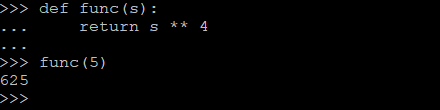
\includegraphics[width=0.5\textwidth]{func.PNG}
\end{figure}


\subsubsection{Information About  the  Function} \label{help_function}
Functions can carry some information and with the use of \texttt{help()} function, we can access to them. For example
\lstinputlisting[language=Python]{help_func.py}
Note that when the information printed it says: Help on function \texttt{name\_of\_function} in module \_\_main\_\_:
this means that it is a function of the file that is currently run.
\subsection{Method}
Methods are functions that are defined on an object. Everything that can be saved in a variable is an object. Some classes of objects are already defined in python, such as strings, floats, integers, lists. About the concept of \textit{class}, look at \ref{class}. The definition of  a class tells which methods are defined on the objects. The concept of  method have similarity with the concept of function, however, it can be considered as particular functions that works on specific objects.  Each object belongs to a class. In other word, objects are instances of a class. Classes are generalisation of objects. They define what information the type of object contains and which functions can be applied to it. The following example elaborates on that.
\lstinputlisting[language=Python]{method_call_example.py}

\subsubsection{Help on method}
To find out the available functions for a particular method, look at the following code.
\lstinputlisting[language=Python]{method_help.py}





\subsection{Output}
You can output text to the console (in case you use a script or interactive python) or under your current cell (in case you use a notebook) by typing print(). You need to add what you want to output between the brackets. It can be a variable or a string, a number, etc.
You can also output multiple things in one line, by separating them by comma.


\subsection{Input}
\label{subsec:Input}
You can input the data in your code using the keyboard. To do so, you just need to use input function: input(). However, you can specify the type your input with another function. Note that the input function would return string.
Example:
\lstinputlisting[language=Python]{input.py}


\subsection{Conditional Statements}
This code shows how to write conditional statements:
\lstinputlisting[language=Python]{if-statement-example.py}
The indented parts are only run under a certain condition.
It is also possible to include more branch options using elif:
\lstinputlisting[language=Python]{if-statement-example2.py}is


\subsection{while-loop}
While loop does a task which is repetitive, and that is very useful if you want to avoid repeating the same piece  of code over and over again.  With while loop you can tell the program how many times the same task should be repeated. 
For instance to compute the factorial of a number we need to multiply all bunch of the numbers below the number and the number itself. This can be done by the while loop more easily. The while loop will go over the same task as often as we want to. We also use the while loop in the occasion where we do not know how often we are going to repeat the same task until we give an input to the code. While-loops can also be
nested, that means the body of a while-loop can contain further while-loops.
\lstinputlisting[language=Python]{factorial.py}
Here is another example where the input number is going to be repeatedly typed until it reaches the number itself
\lstinputlisting[language=Python]{repeat.py}
\subsubsection{while-True}
Here is an example which can show how can we have an open loop while code. It basically means that the loop continues non-stop unless we want to break it. For example in the following code we can input as many integer number as we wish and once we enter \texttt{q}, it gives us the sum and the product of the numbers.
\lstinputlisting[language=python]{sum_product.py}


\subsection{for-loop}
Unlike a while-loop, a for-loop does not run until a specified condition is met, but rather runs over sequential
data types and runs its body for every element in that sequence.  Therefore it is particularly useful to traverse
sequences.  It can also be used in combination with range.
\lstinputlisting[language=Python]{for_loop.py}
\subsubsection{list comprehension}
\label{list_comprehension}
We can use for loops to convert one list into another. But there is an easier way of doing that, which is called list comprehension. We create a list, where the elements are defined relative to a for loop.
\lstinputlisting[language=Python]{list_comprehension.py}
\subsubsection{nested for-loop}
\lstinputlisting[language=Python]{nested_for_loop.py}

\subsection{Sets}
A set is a collection that does not store the order nor the number of appearances of objects. The objects in a set are called members of the set.  It stores element, however, it only stores which elements belong to the set. It does not store how often an element belongs to a set or where in the set it is positioned. Sets also implement various operations of set theory (mathematics), such as ``difference", ``issubset", ``issuperset", ``isdisjoint", ``union" or ``intersection", etc. The set can find out if an element is there because it can internally sort the elements and can do that simply because it doesn't need to preserve the order in which the elements are given. Searching in sorted structure is faster than searching in an unsorted structure. Example
\lstinputlisting[language=Python]{set.py}
\subsubsection{Use-cases of sets}
The membership query operator, \texttt{in}, is also available for lists. The advantage of using it on sets is that the query runs faster. This is because the set can store the data internally in a way that helps it find the elements faster (for example in some sorted structure), because it does not have to preserve the order of the elements. If the membership of elements is queried relatively often, then it is useful to store the elements in a set. Note that converting a list to a set also takes time.

\subsection{Dictionaries}
A dictionary is a data-structure that allows to look up values associated to keys. Example:
\lstinputlisting[language=Python]{dictionary_example.py}
\subsubsection{Iterating through dictionaries}
We can use a for loop to iterate through the keys of a dictionary, just like through a list. For each element, we can access the associated value. See the following example:
\lstinputlisting[language=Python]{dictionary_iteration.py}
\subsubsection{Dictionary Comprehension}
Similar to lists (described in \ref{list_comprehension}), we can also use a systematic way of constructing dictionaries in one line of code. We call this "dictionary comprehension". Example:
\lstinputlisting[language=Python]{dictionary_comprehension.py}
\subsubsection{Find key for minimum (maximum) value}
In many applications, it is useful to find the element that has the highest (or lowest) associated value. We can also sort dictionaries by value. Example:
\lstinputlisting[language=Python]{dictionary_min_max.py}


\subsection{Zip}
Sometimes you want to compute a number of values based on two lists of values. In this case, a simple list comprehension is not sufficient, because you can only iterate through one of the lists. An appropriate solution for this problem is the zip function. It takes several lists (you can choose as many as you like) and creates one list of tuples where the ith element is from the ith list and their order is the same as in the original lists. Example:
\lstinputlisting[language=Python]{zip_example.py}
\subsection{Exception handling}
Sometimes depending in data, a python command can cause errors. In a script you would want to avoid errors if you can foresee them. This is useful, because errors usually stop the program. The following two examples  can illustrate the concepts better. First we present a code which cause an error.
\lstinputlisting[language=Python]{error.py}
Now, we foreseen the error.
\lstinputlisting[language=Python]{except.py}
\subsection{Tuples}
It is often practical to store values that belong together in the same variable. This becomes particularly useful if you want to return multiple values from a function. The function can then simply return a tuple. A tuple can be created by writing variables behind each other, separating them by commas and surrounding all by round brackets. For example:
(2,10).
The individual values of a tuple can be accessed either by treating the tuple like a list:\\
first\_value = my\_tuple[0]\\
second\_value = my\_tuple[1]
\\
Or by assigning the tuple to multiple variables:
first\_value, second\_value = my\_tuple
\\
In the following code, we use tuples to return two values from a function:
\lstinputlisting[language=Python]{multi_return.py}
Note that in this code, we are using the concepts of enumerating a list, which      itself is a function that returns two values and is described in section \ref{enumerate}. The test code for this function is only run if the file itself is run, not if it is imported, because we use the main condition (\ref{main}).
\subsection{Class}
\label{class}
We have learned about data types of Python in section \ref{subsec:data_types}. Each of these and more data types are implemented by a construct called class. We can also define our own classes for custom data types. In the following example, we write our own data type called time, which is a blueprint of how times work.
\lstinputlisting[language=Python]{class.py}
The purpose of a class is to make instances of it. We do that by defining a name of the instance and type assign the name of the class followed by (). Each class can have \textit{methods}. Methods are similar to functions but they are defined in the class definition, and are referring to an instance of that class (that means an object of that class). They can tell us about the content of the instance or modify it. We call them by typing the name of the instance dot the name of the function, as shown in the example.
It is also possible and often necessary to query which class an object belongs to. We can do that by using the function ``type".
\\
Find a simpler example in section \ref{subsec:init}.


\subsection{Write Data out to Files}

We have used function for writing file which belongs to numpy package that we discuss later. 
We can open a file in python and write into it, here is an example
\lstinputlisting[language=python]{write.py}
As an alternative way to write in a file using numpy we can use the following code.
\lstinputlisting[language=python]{save.py}
\lstinputlisting[]{ourdata.txt}

\subsection{Read Data in from Files} 
For reading data into python we can also use \texttt{open()} function for reading, as an example 
\lstinputlisting[language=python]{read.py}
There is also other alternative that works with numpy, but it requires file to be formated just like \te{savetxt()} formats it.  Here is an example
\lstinputlisting[language=python]{read2.py}
Note that, your file that is going to be loaded or be written in it, doesn't necessary have to be in the same folder that the code is. We can also give a path to the directory of the file either absolute path or relative.
\subsubsection{Read in Several Data files}
Here is an example on how to read several data files using \te{glob}.
\lstinputlisting[language=python]{several_read.py}
If we want to manipulate the data, pandas makes it convenient.
The pandas is a package explained in detail in section (\ref{pandas}). Here we show how we can read in data using pandas. Here is an example on how to read several .csv files using pandas. In this example we read in all the files containing COVID-19 total cases for different dates. In this case there are two of them.
\lstinputlisting[language=python]{read_several_pandas.py}

\subsubsection{Uploading files in google colab}
Here we explain two ways that we can upload a file to google colab. When you run a colab notebook, a separate file system is created on the server. This is called a session. It stores the files that we can read into our code and those that we write in our code. If we have a file on our computer that we want to use in colab, we can either upload it directly into that file system, or upload it to Google Drive and then mount our Google Drive folder into the file system.
In order to upload a file from your local system to google colab, we can use this code:
\lstinputlisting[language=python]{file_upload_1.py}
Alternatively, we can upload the file to Google Drive, and then mount our Google Drive into the colab session. The following code assumes that we have uploaded the file already, so it just shows the mounting:
\lstinputlisting[language=python]{file_upload_2.py}

\subsection{import}
We can import files as we import libraries into a python code, and we can also import a part of a code like functions that is initially written in an old file. The old file (or the file whose  content is being imported) can be called as a module \footnote{a collection of modules can make a library or package}. Let's import a simple example where we defined a function in another python file and now we would like to use that in our new python file so we need to import that. Here is the file that we create for having the function we want to import
\lstinputlisting[language=Python]{func2.py}
here is the file that imports our function and uses it.
\lstinputlisting[language=Python]{import.py}
As you notice, when we run import.py, the output is not only the result of the function that we call for, but also the result of the file which contains that function. To avoid that we need to learn about \textit{main condition}, which we have explained in \ref{main}. And the appropriate codes for our new file is as follows.
Here is the change that we need to make for the main file which contains the function.
\lstinputlisting[language=Python]{func3.py}
here is the result that we expect.
\lstinputlisting[language=Python]{import2.py}

\subsection{Packages}

There are plenty of useful functions and methods written for python, however, not all of them are installed by default. Packages are collections of modules, which includes functions, methods etc for specific purposes.  Based on the requirement of the users they can be installed and being used. The packages are abundant and makes no sense to include them in python initially, and also they are under constant development, therefore, anyone who wants to develop or use a package, they need to install them first. Here is a simple way of installation (a package called NumPy)  using \texttt{pip}:
\begin{enumerate}
\item go to this link \href{https://pip.readthedocs.io/en/stable/installing/}{https://pip.readthedocs.io/en/stable/installing/}
\item download \texttt{get-pip.py}
\item go to the terminal:
\begin{itemize}
\item type: \texttt{python3 get-pip.py}
\item type: \texttt{pip3 install numpy}
\end{itemize}
\end{enumerate}
If you want to figure out the defined functions, etc inside the packages, you can use \texttt{dir()}. For instance, if you want to get into NumPy package, you can type \texttt{print(dir(numpy))}, provided that you already imported NumPy. 

%See the followoing: \lstinputlisting[language=Python]{dir.py}



Note that we can also import a sub-package from a package, one example is when we import pyplot sub-packeage from matplotlib package,  \texttt{matplotlib.pyplot}. See \ref{plot_list}.
The official documentation on how to make packages and modules of your own can be found \href{https://docs.python.org/3/tutorial/modules.html}{here}. Here is also an interesting blog to learn more about 




%%%%%%%%%%%%%%%%%%%%%%%%%%%%%%%%%%%%%ADVANCE %%%%%%%%%%%%%%%%%%%%%%%%%%%%%%%%%%%%%%%

\section{Advanced}
\subsection{$\ast$args}
So far we have written functions and methods that receive specified number of parameters. Now, we learn how to make functions receiving arbitrary numbers of arguments. Example:
\lstinputlisting[language=Python]{args.py}
\subsection{$\ast\ast$kwargs}
There is a second option to pass an arbitrary number of arguments: If we add two $\ast$ in front of the parameter, it becomes a dictionary. We are then supposed to provide a name for every one of the parameters that we give - we get an error otherwise. Example:
\lstinputlisting[language=Python]{kwargs.py}








%%%%%%%%%%%%%%%%%%%%%%%%%%%%%%%%%%%%%NUMPY %%%%%%%%%%%%%%%%%%%%%%%%%%%%%%%%%%%%%%%%


\section{NumPy}
\href{https://numpy.org}{NumPy} is a library that brings many functions and data structures that are useful for scientific computing in general and matrix computing in particular. 

\subsection{numpy arrays}
we can arbitrary make an array of numbers, see the following
\lstinputlisting[language=Python]{array.py}
\label{subsec:numpy_arrays}
NumPy deals with arrays and matrices. In the following example you can see how an operation on a list differs from the numpy array.
\lstinputlisting[language=Python]{numpy_ex1.py}
Elements in the numpy array can be any types, however if the types are different from one another, then one type would be the type of the array we set, that means all the elements are converted to the same type. Python  decide which type will that be. For instance, if you use mix of integers and strings, the string would be the final type of all elements. Also note that when you initially decide on which type you want to create your array, and later you if you insert  an element within the array with different type, the type of the new element would be converted to the  original type of the array, if possible. Look to the following examples.
\lstinputlisting[language=Python]{numpy_ex2.py}
A side note: If you insert integers, strings, and booleans in a numpy array, you get to have a single type of string.
Note that the property of the NumPy array which requires it to hold elements of a single type makes the NumPy faster in calculation compared with list. Also note that if you have a numpy array with booleans and number types (float, integer), numpy will convert the boolean \texttt{True} to 1 and \texttt{False} to 0.
\subsection{slicing}
Slicing means accessing a subsection of a numpy array.
The following examples can represent how it works
\lstinputlisting[language=Python]{slicing.py}


\subsection{shape and reshape}
Here is we introduce the reshape function, which can change the dimensions of the numpy array. Here is some examples
\lstinputlisting[language=Python]{reshape.py}


\subsection{linspace}
Linspace function is being used to create a line with the amount of discretization that we would like to have. For instance, if we want to have a 20 meters stick and we want to chop it 100 times, each piece would have 0.2 meter length, this can be useful in some problem. This example can be seen in the following code
\lstinputlisting[language=Python]{linspace.py}


\subsection{arange} \label{arange}
Arange is a function that generate arrays with desired space between the elements. It is similar to linspace with the difference that the last number would indicate the size of the steps rather than the number of the steps. It works exactly like range, except that it makes numpy array. Look at \ref{range} The following examples would elaborate on it better.
\lstinputlisting[language=Python]{arange.py}


\subsubsection{comparing arange and linspace}
In this example we can see the difference between arange and linspace more clearly.
\lstinputlisting[language=Python]{linspace_and_arange_comparision.py}


\subsection{meshgrid}
Meshgrid can help us to find the coordinates of a certain point in a multi-dimensional space. It takes input arrays that can be seen as coordinate axes. Let's assume we give two arrays. These form the coordinate axes of a two-dimensional space. Meshgrid tells us the coordinates for each position in the resulting two-dimensional array. Each position has (in the two-dimensional case) two coordinates. So meshgrid retuns two two-dimensional arrays, one with all the coordinates in the first and the other in the second dimension. A good visualisation is shown under the following 
\href{https://browse.startpage.com/do/show_picture.pl?l=english&rais=1&oiu=https%3A%2F%2Fi.stack.imgur.com%2F8Mbig.png&sp=68ba4eb553807530320e70250d5a4696&t=default}{link}:
Here is how it works in a two dimensional arrays which is representing the link's example.
\lstinputlisting[language=python]{meshgrid.py}


\subsection{random}
Here we illustrate how to generate random numbers using numpy
\lstinputlisting[language=Python]{random1.py}


\subsection{hstack()}
hstack function can be used to stack data horizontally, for example
\lstinputlisting[language=python]{hstack.py}


\subsection{vstack()}
\lstinputlisting[language=python]{vstack.py}
\subsection{Conditional Selection}
The following example will illustrate how we can select elements of a numpy array that meet a certain condition. 
\lstinputlisting[language=python]{numpy_condition.py}
Here you can find another useful code on picking the right data from the second numpy array.
\lstinputlisting[language=python]{statistic1.py}


\subsection{np.where}
this function can be used to apply an operation on elements of numpy array. Here you can find an example where it returns the absolute value of a list of numbers.
\lstinputlisting[language=python]{where.py}

\subsection{Statistical Methods}
Here is some Numpy function that can be useful dealing with data. 

Functions like: mean, median, min, max. 

\lstinputlisting[language=python]{statistic.py}


\subsection{Error with math versus numpy}
We have seen that basic arithmetic operations, such as addition or multiplication, can be performed on numpy arrays and apply to every element. Some mathematical operations are implemented as functions in the math package, such as \te{sqrt(), sin(), cos(), and etc}. These do not work on numpy arrays. When you give numpy ad parameter to them it throws the following error. Look at the file

\lstinputlisting[language=python]{numpy_and_math_error.py}

We have found one solution for it, and that is using the functions from numpy package not from math package.

\lstinputlisting[language=python]{numpy_math_fix.py}










%%%%%%%%%%%%%%%%%%%%%%%%%%%%%%%%%%%%% MATPLOTLIB %%%%%%%%%%%%%%%%%%%%%%%%%%%%%%%%%%%%%%%%


\section{Matplotlib}
Matplotlib is a library that allows to represent data graphically. The plenty of examples provided in \href{https://matplotlib.org/gallery/index.html}{this link} can help a lot while trying to plot your favourite one. Also the tutorial \href{https://python-course.eu/matplotlib.php}{here} can be useful.
Here we check some of them. Along with simple examples we try to show some of the features that you can add to a plot.


\subsection{Plotting List of Data} \label{plot_list}
here is a simple example for a one-dimensional list
\lstinputlisting[language=Python]{plot_list_data_1.py}
The result looks as follows
\begin{figure}[h]\centering \caption{one-dimensional plot}
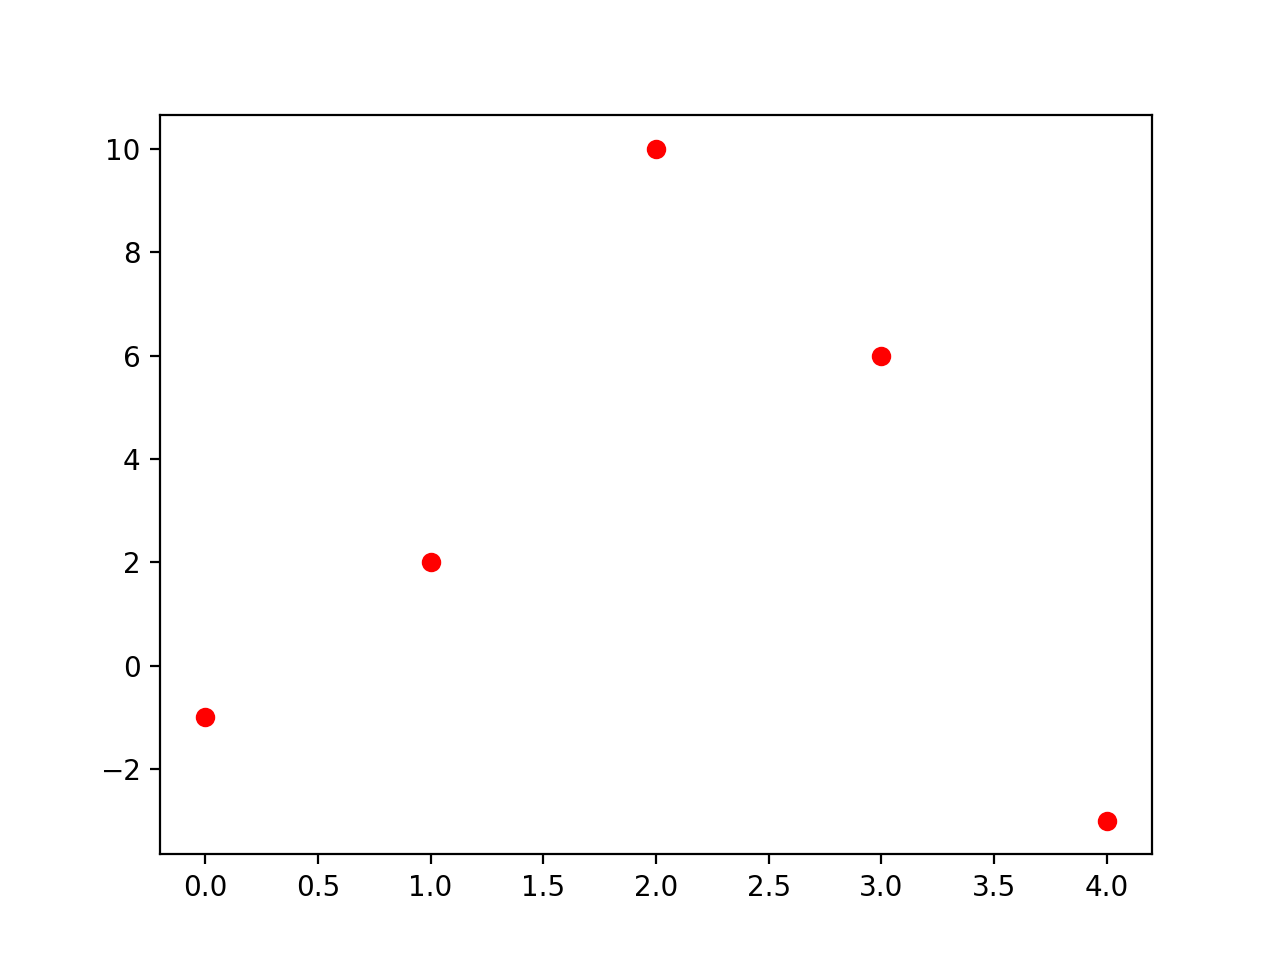
\includegraphics[width=0.5\textwidth]{plot_list_data_1.png}
\end{figure}
As you see the vertical axes is the range of our data and the horizontal axes varies with step one by default. 
Here is the two-dimensional version of the plot
\lstinputlisting[language=Python]{plot_list_data_2.py}
The result looks as follows. 
\begin{figure}[h]\centering \caption{two-dimensional plot}
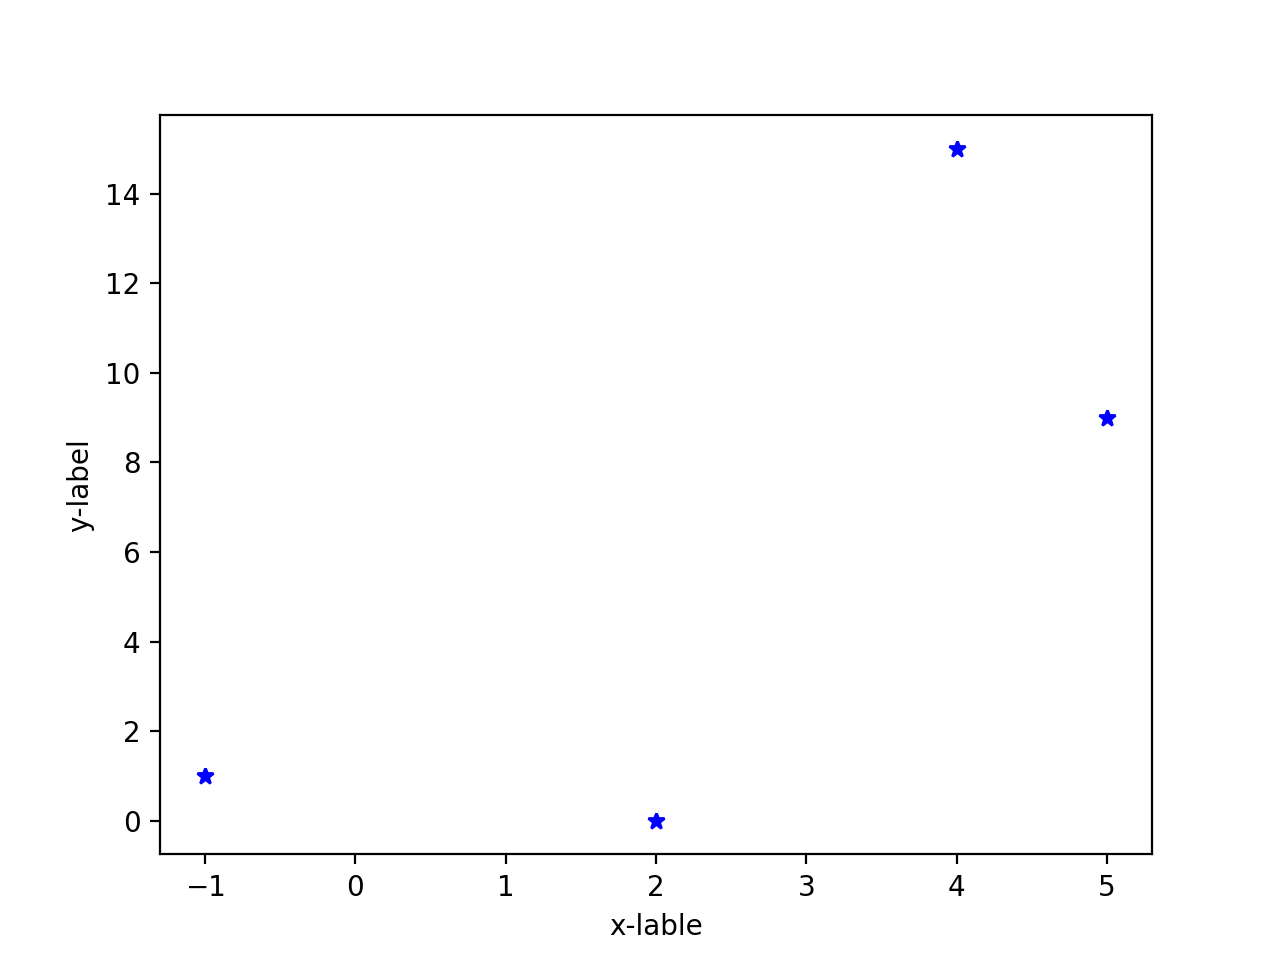
\includegraphics[width=0.5\textwidth]{plot_list_data_2.png}
\end{figure}
You can obtain the two dimensional plot also with the scattering option. Note that, scatter plot is useful to assess the correlation between horizontal and vertical axes's.
\lstinputlisting[language=Python]{plot_list_data_3.py}

\begin{figure}[h]\centering \caption{scatter plot}
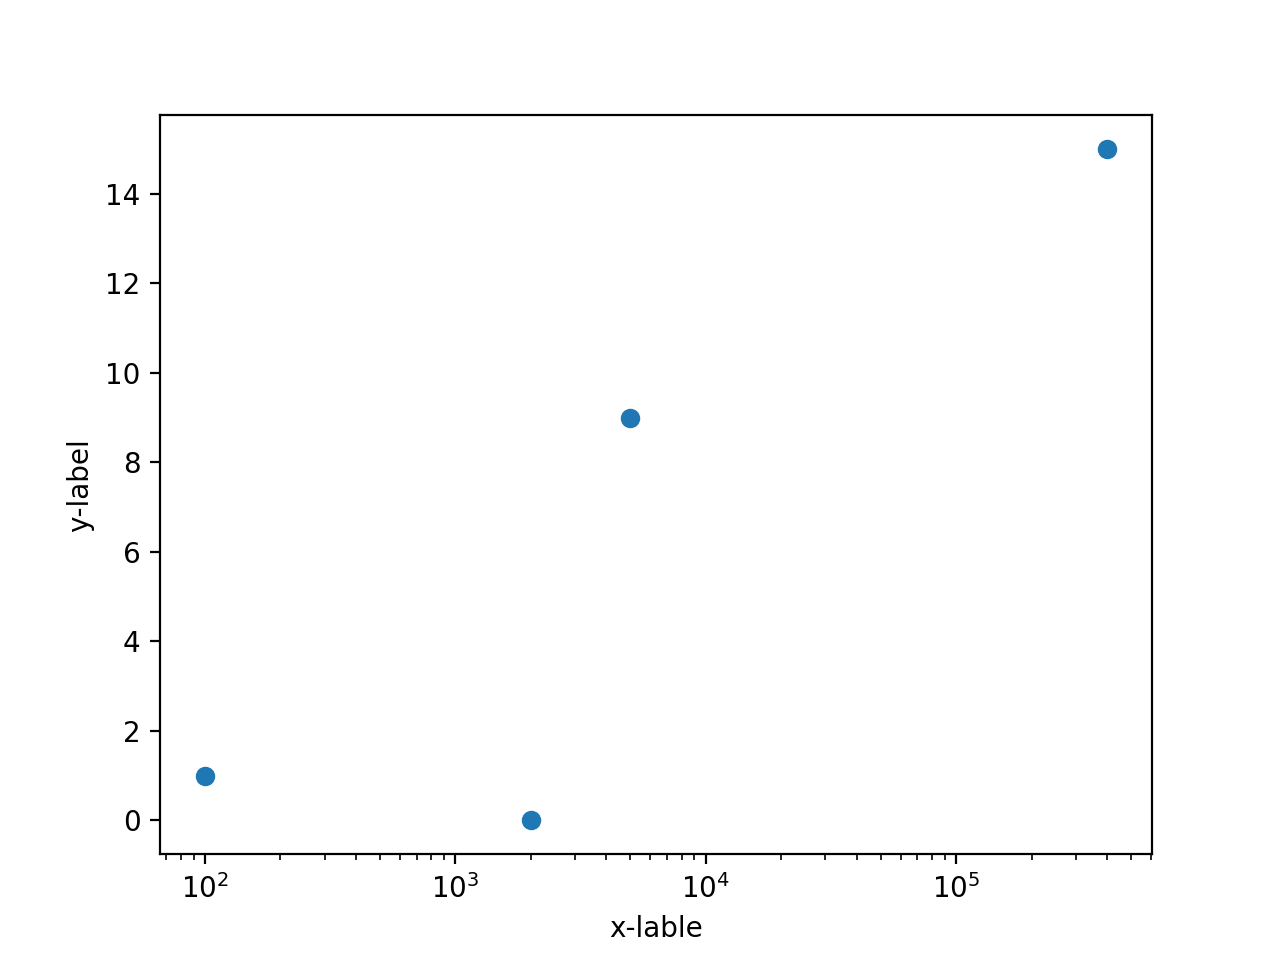
\includegraphics[width=0.5\textwidth]{plot_list_data_3.png}
\end{figure}

\subsubsection{connected data point list plot}
\lstinputlisting[language=Python]{plot_list_data_4.py}
\begin{figure}[h]\centering \caption{connected points (line plot)}
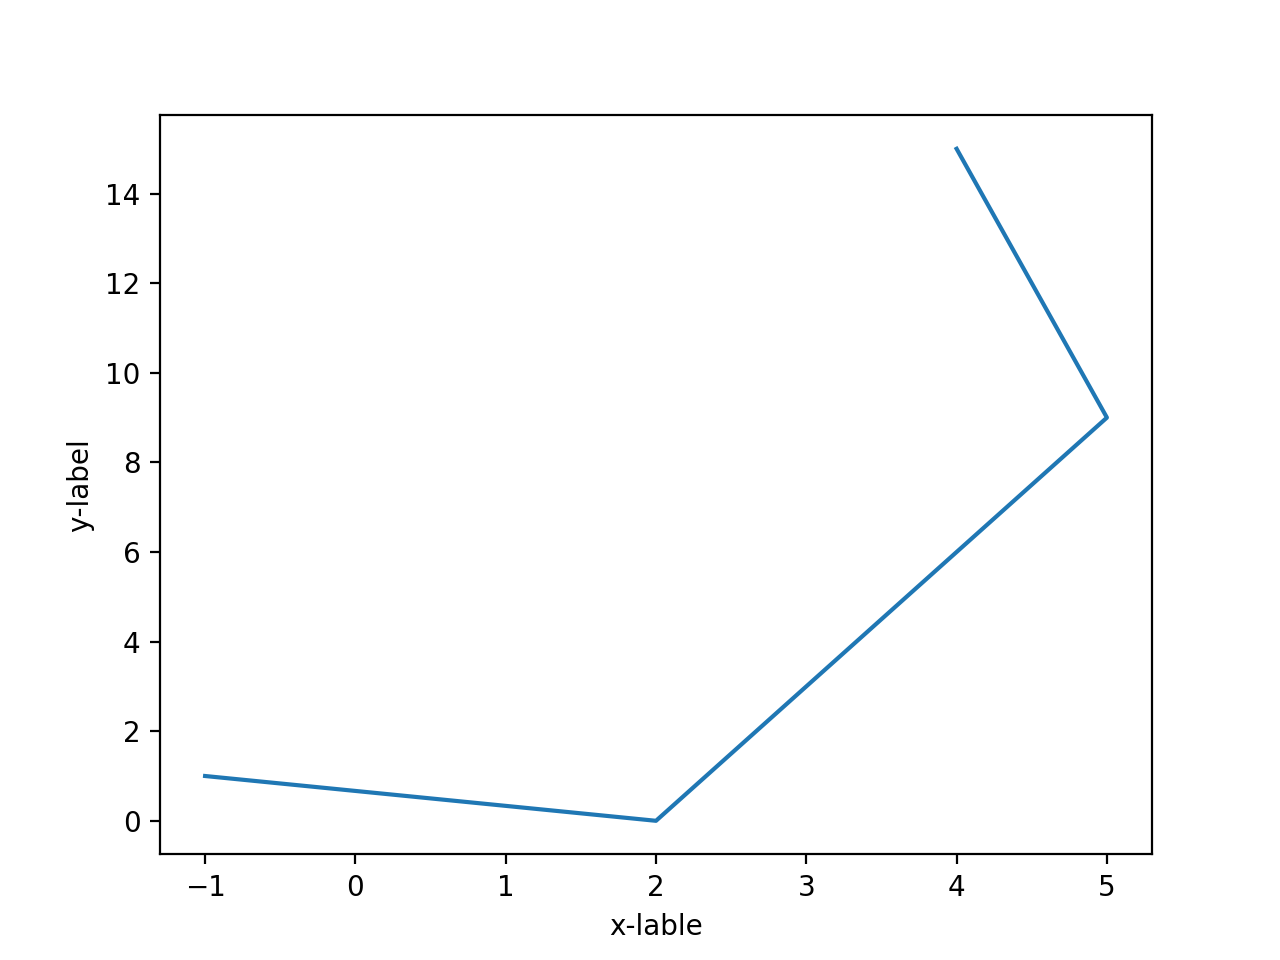
\includegraphics[width=0.5\textwidth]{plot_list_data_4.png}
\end{figure}

\subsection{Plotting Function}
Here is a simple example how to plot a $\sin(x)$ function.
\lstinputlisting[language=Python]{sin.py}
\subsection{3D plot}
\lstinputlisting[language=Python]{3dplot.py}
\begin{figure}[h]\centering
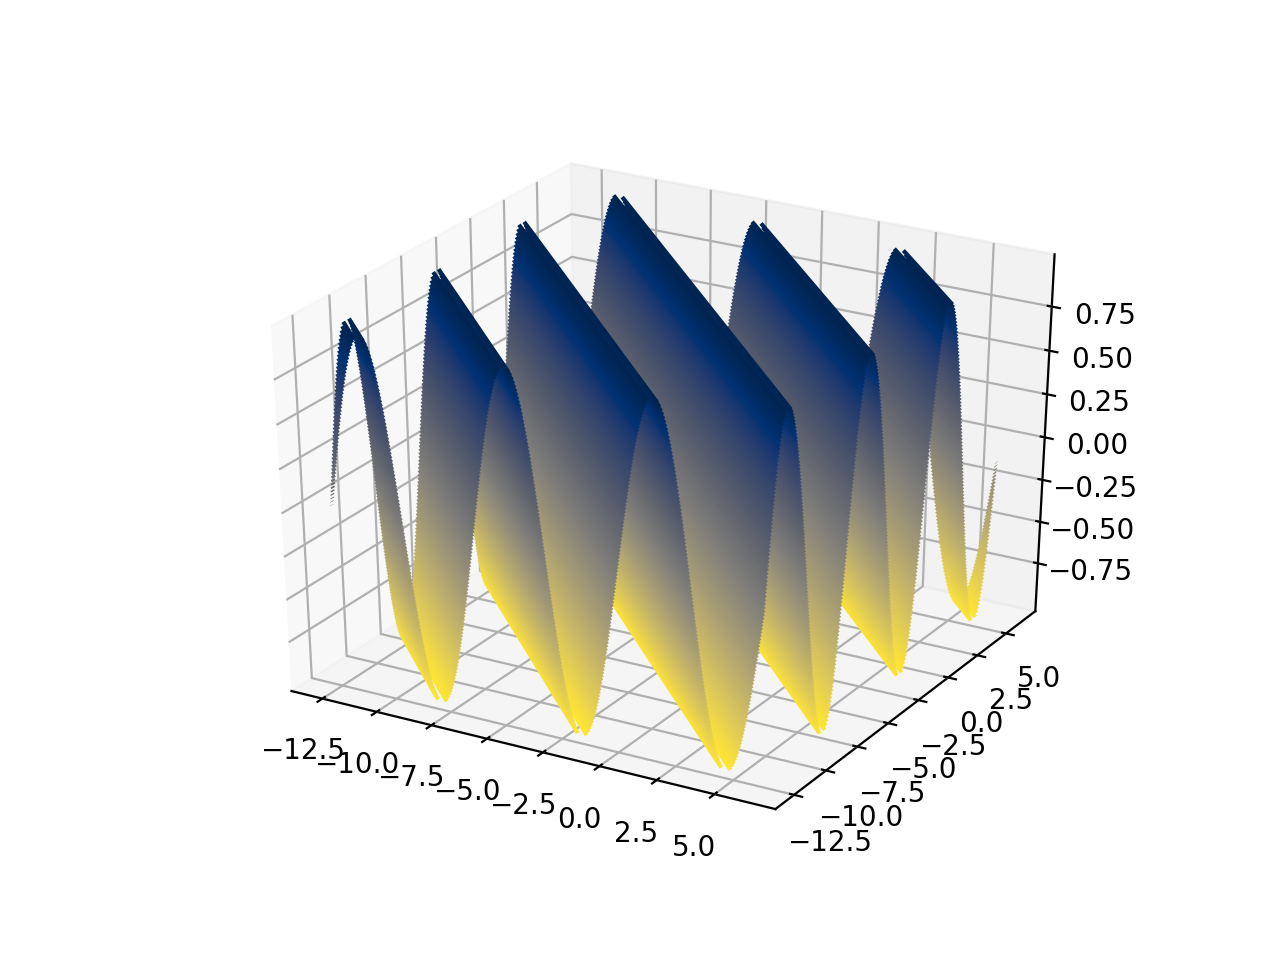
\includegraphics[width=0.6\textwidth]{3dplot.png}
\end{figure}
\begin{figure}[h]\centering
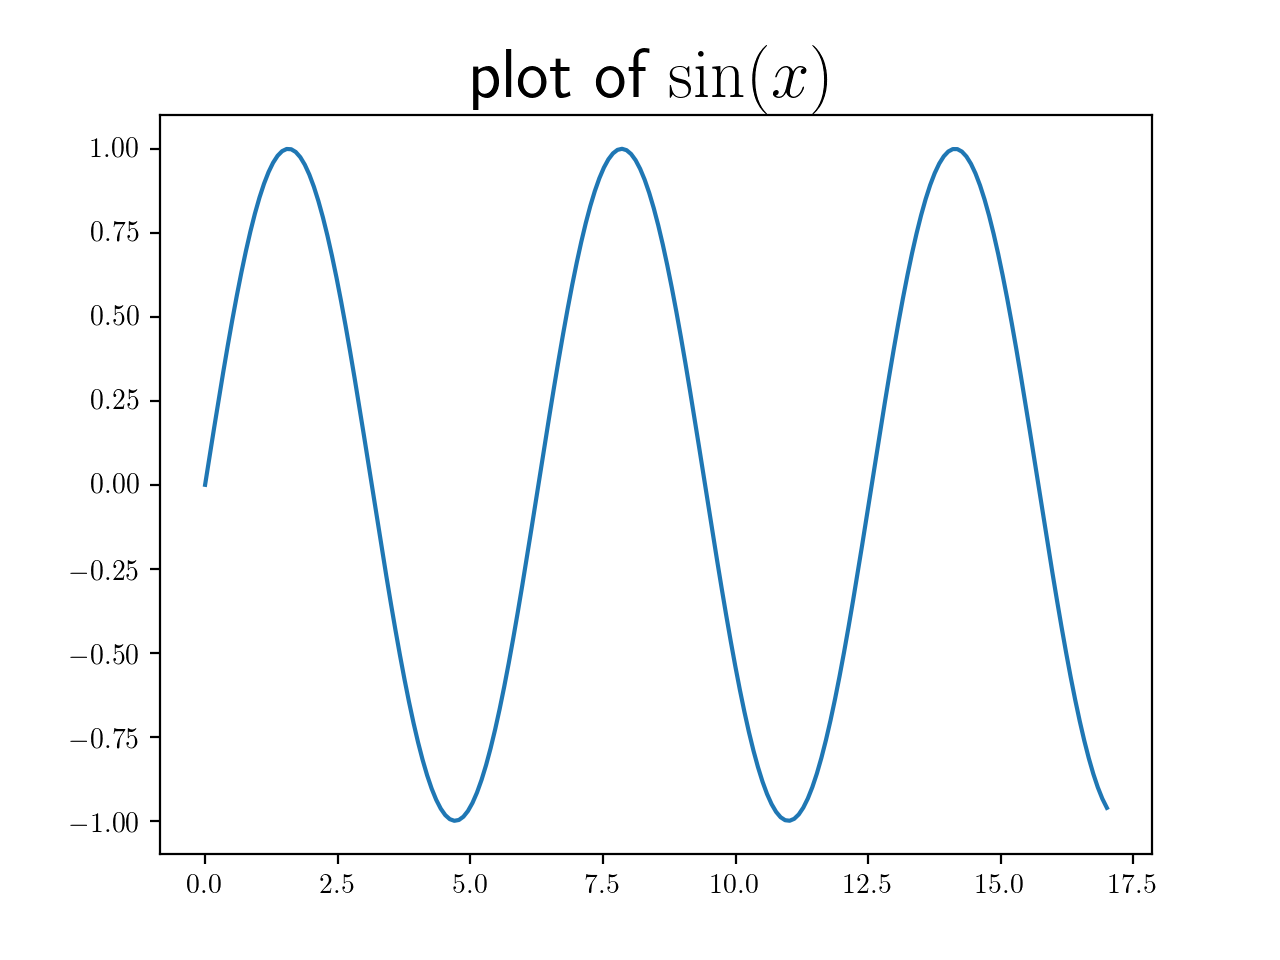
\includegraphics[width=0.5\textwidth]{sin.png}
\end{figure}
\subsubsection{Extra remark on plotting functions}
Note that there are cases that \te{math} functions would not work properly with numpy. In this case we can either use the numpy functions or vectorization technique. 
Let's take a look at this example:
\lstinputlisting[language=Python]{plot_error.py}
One way to simply resolve this is by altering \te{math} to \te{numpy}.
\lstinputlisting[language=Python]{plot_fix.py}
Another way is to use the \te{vectorize} function, see example
\lstinputlisting[language=Python]{vectorisation.py}
\begin{figure}[h]\centering
\caption{vectorisation}
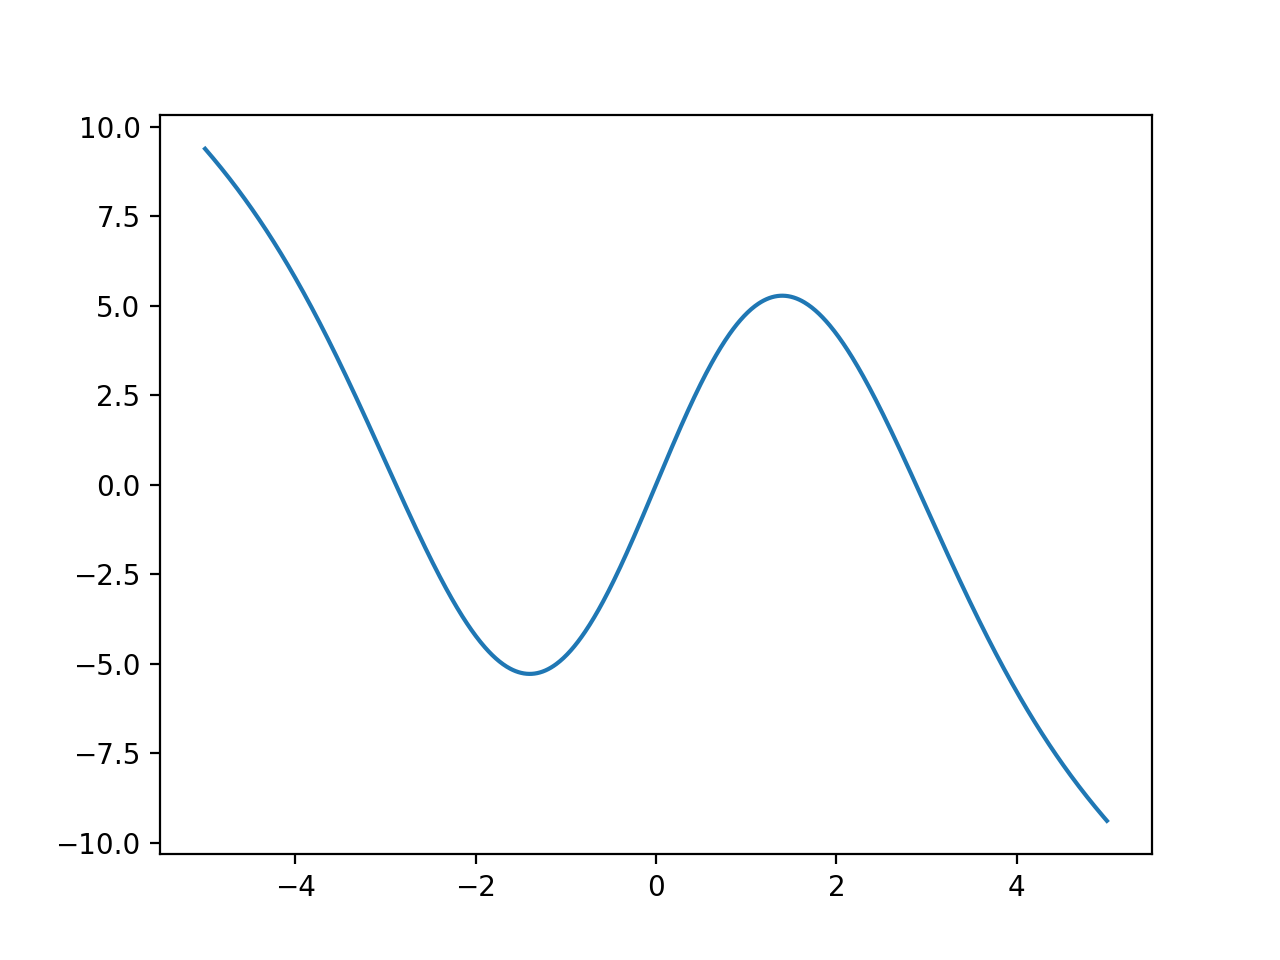
\includegraphics[width=0.5\textwidth]{vectorisation.png}
\end{figure}

\subsection{subplot}
here is an example where we can learn how to make several plot in the same figure.
\lstinputlisting[language=Python]{subplot.py}
\begin{figure}[h]\centering
\caption{here is an example of subplot}
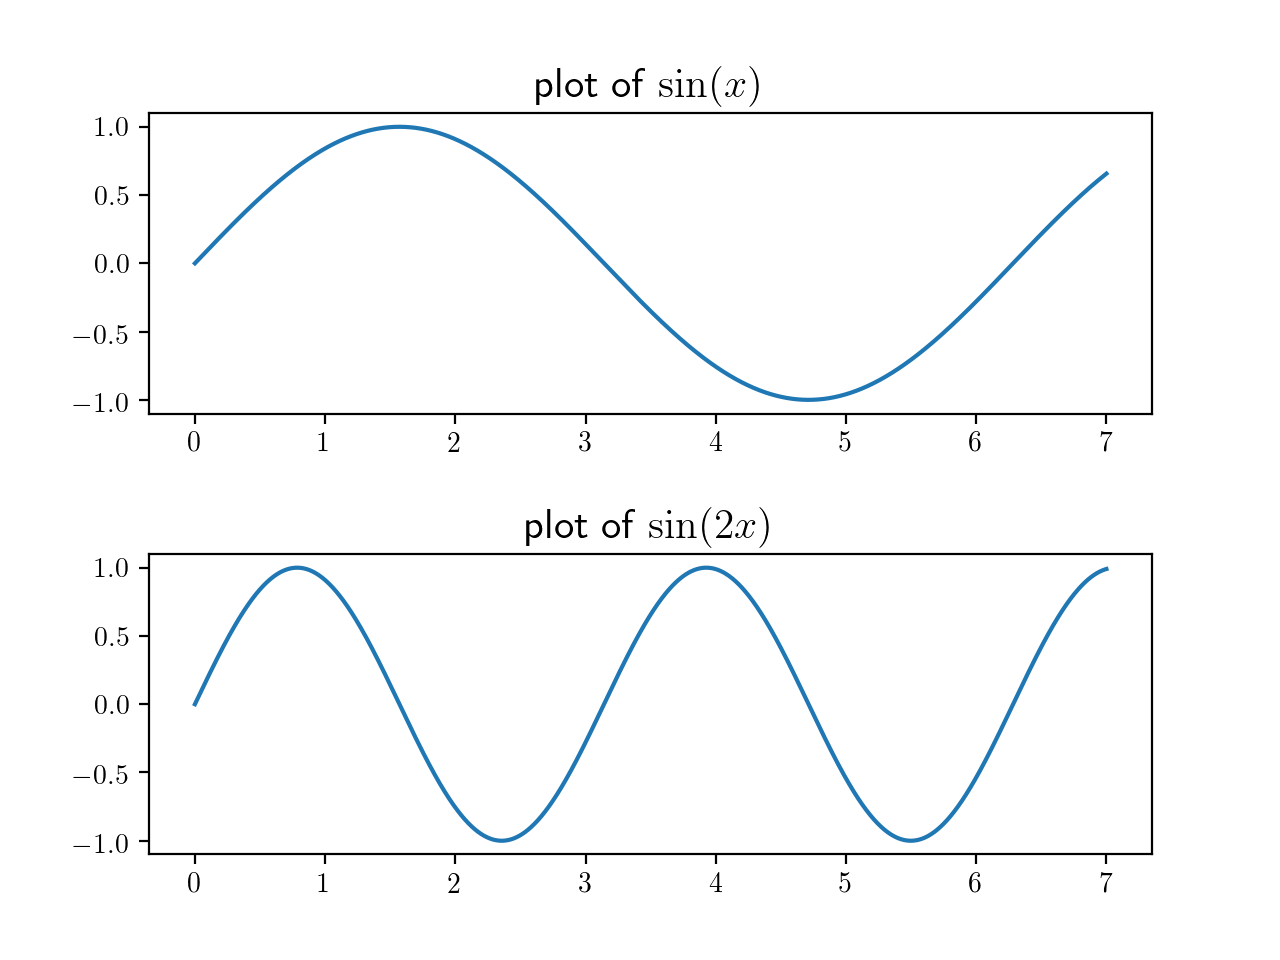
\includegraphics[width=0.5\textwidth]{subplot.png}
\end{figure}


\subsection{Histogram}
Here you can see, one of the simplest example for making a histogram of the data. 
A histogram shows how data is distributed - that means how many  data points appear with values in certain ranges.
The hist-function divides the difference between the highest and the lowest value into bins of equal size. You can specify the number of bins or set it to 'auto' for an automatic decision of how many bins should be made.
To estimate the distribution of the data from the histogram, it is recommended to have roughly sqrt(n)
 bins, where n is the number of data points.
 In the exceptional case that a data value is exactly on the boundary of a bin, it will be counted for the next, not the previous bin, except if it is the largest value, which is counted towards the previous bin. In the example given in this part, you can check how the values are distributed in the boundaries of ranges. 
 In our example, there are 5 bins, each of them having the size 2. So there is a bin for the range 6 to 8 and another one for the range 8 to 10.
\lstinputlisting[language=Python]{histogram.py}
\begin{figure}[h]\centering
\caption{here is an example of histogram}
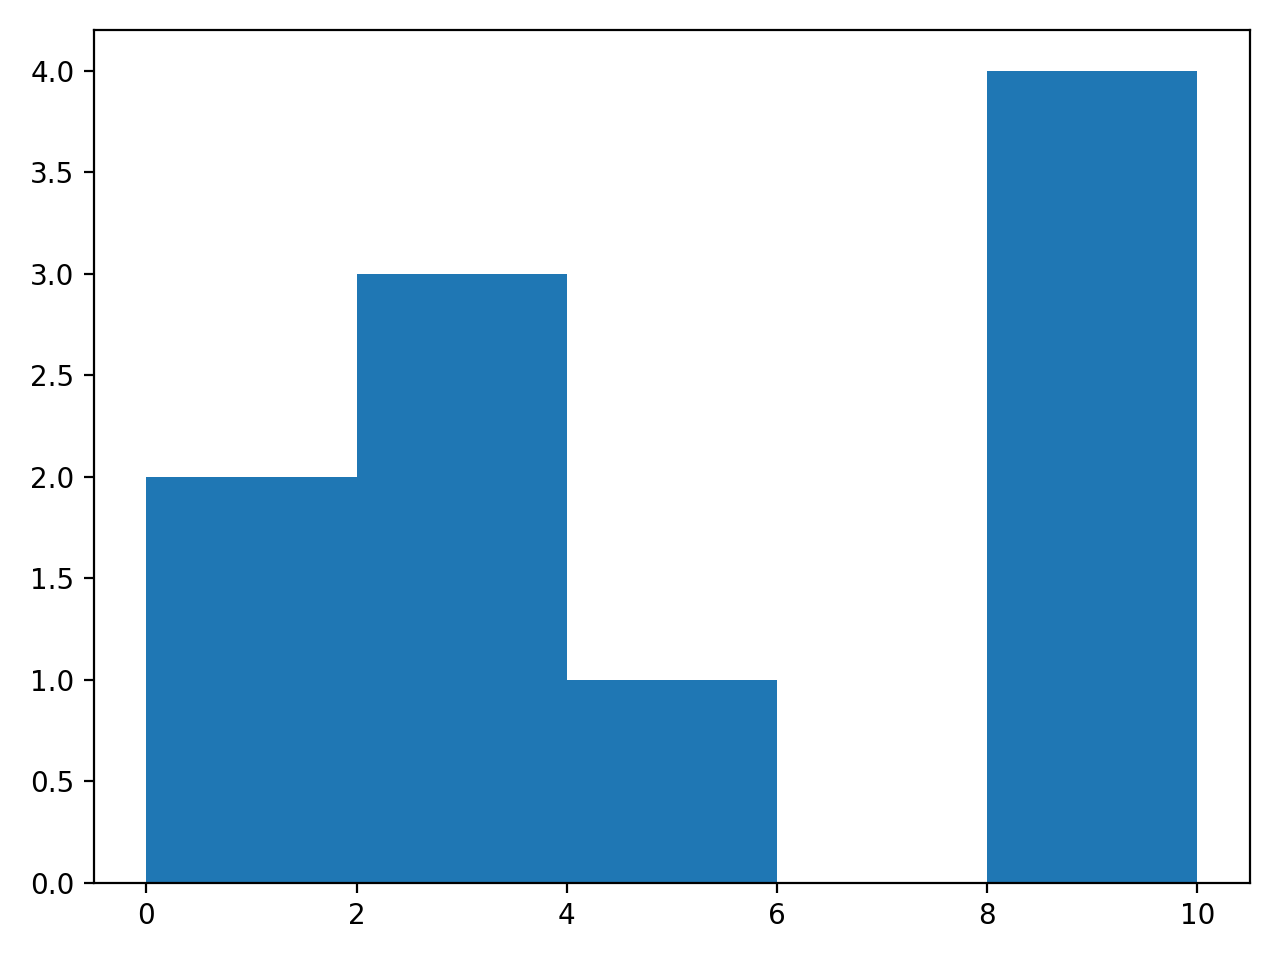
\includegraphics[width=0.5\textwidth]{histogram.png}
\end{figure}



\subsection{Customisation}
In the following plot we see, how fill\_between, and 
yticks/xticks functions work.

\lstinputlisting[language=Python]{fill.py}
\begin{figure}[h]\centering
\caption{fill\_between, and yticks}
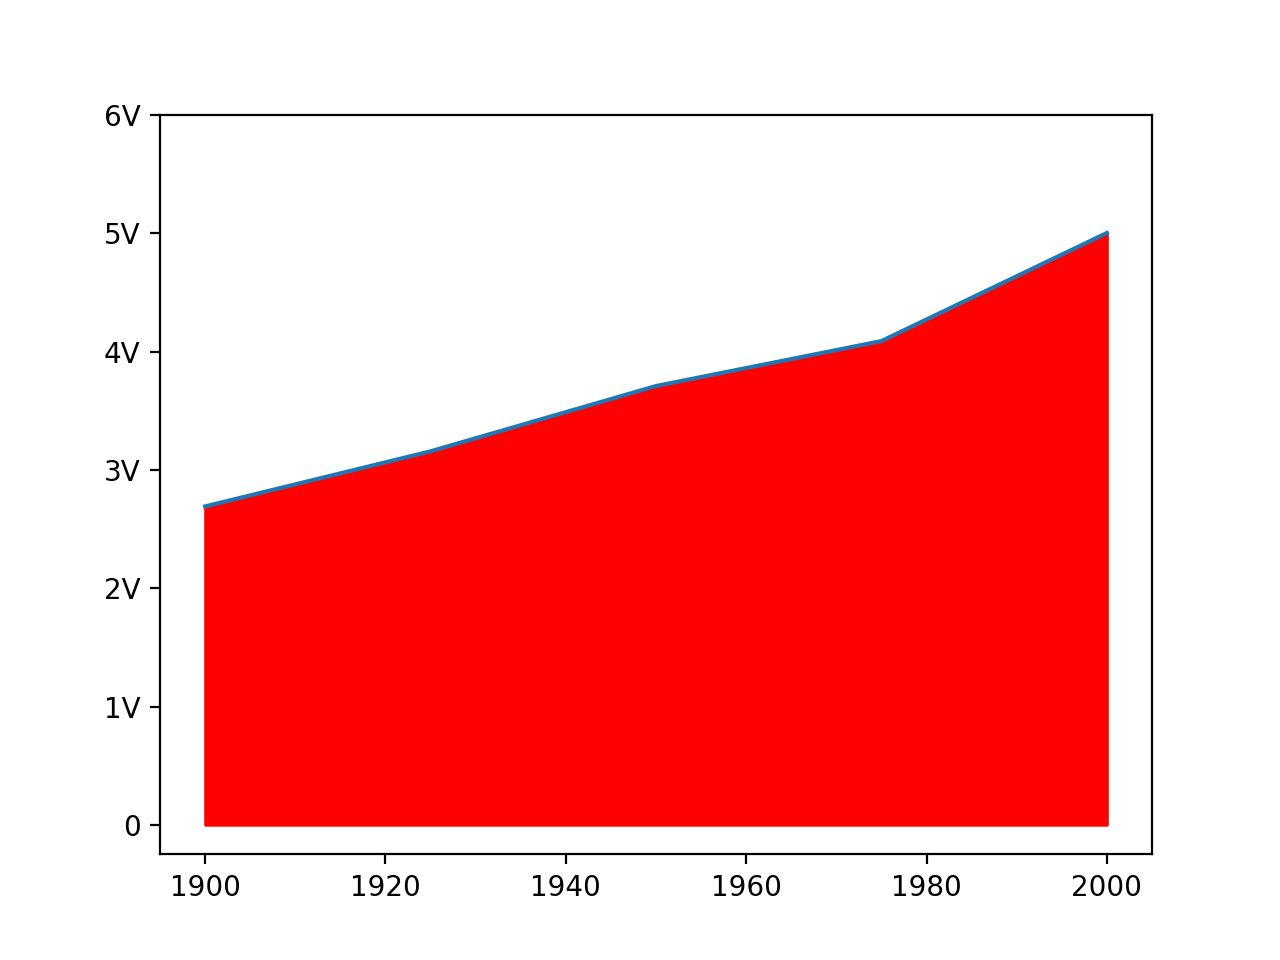
\includegraphics[width=0.5\textwidth]{fill.png}
\end{figure}
Here is an example for the scatter plot with the size of the data points.

\lstinputlisting[language=Python]{scatter_size.py}
\begin{figure}[h]\centering
\caption{scatter plot with size and colors}
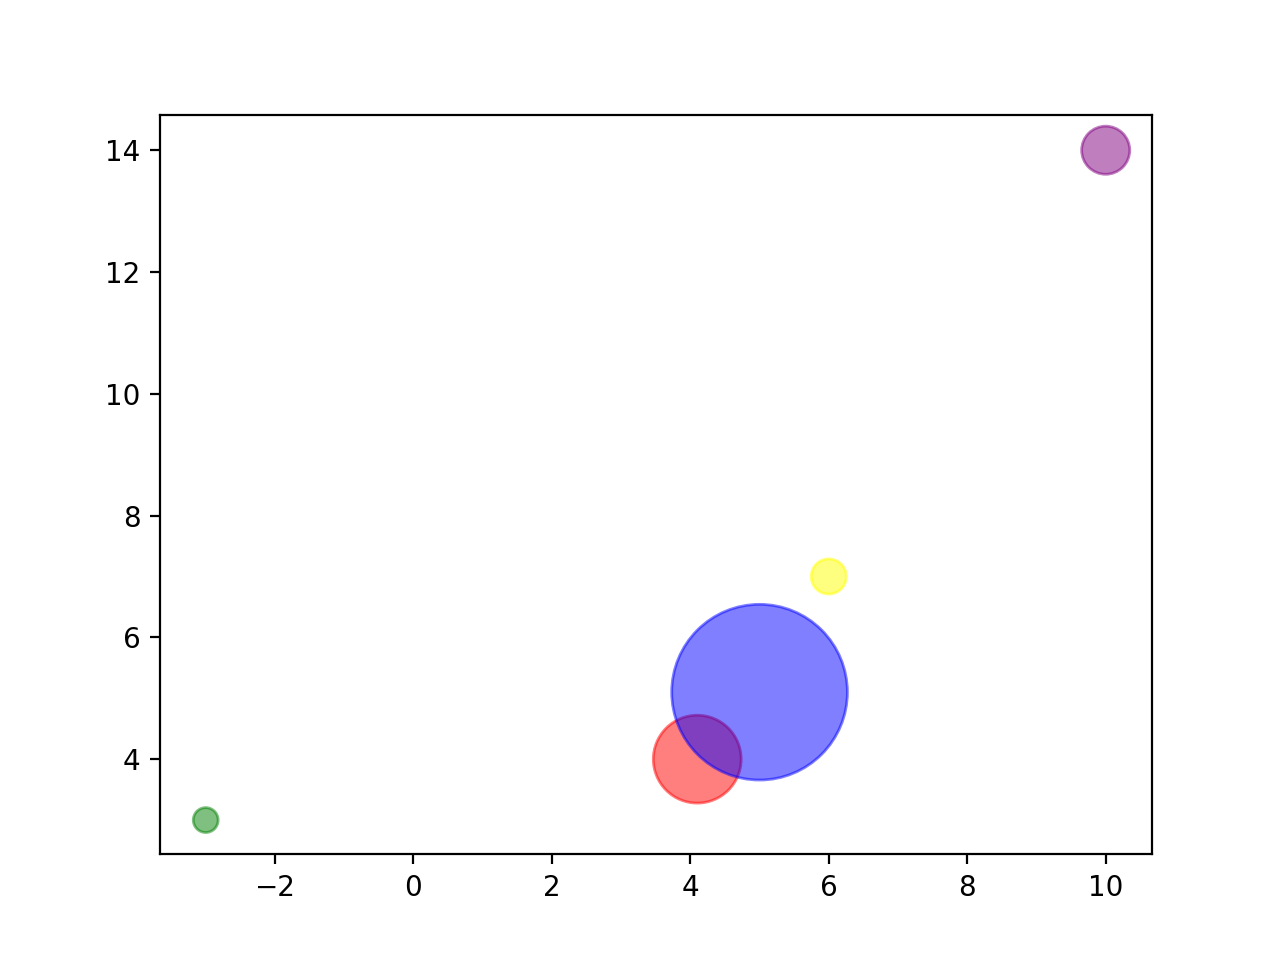
\includegraphics[width=0.5\textwidth]{scatter_size.png}
\end{figure}

\subsection{Legends} \label{legend}
Here is an example on how to make a legend for a plot.
\lstinputlisting[language=Python]{legend.py}
\begin{figure}[h]\centering
\caption{Legend}
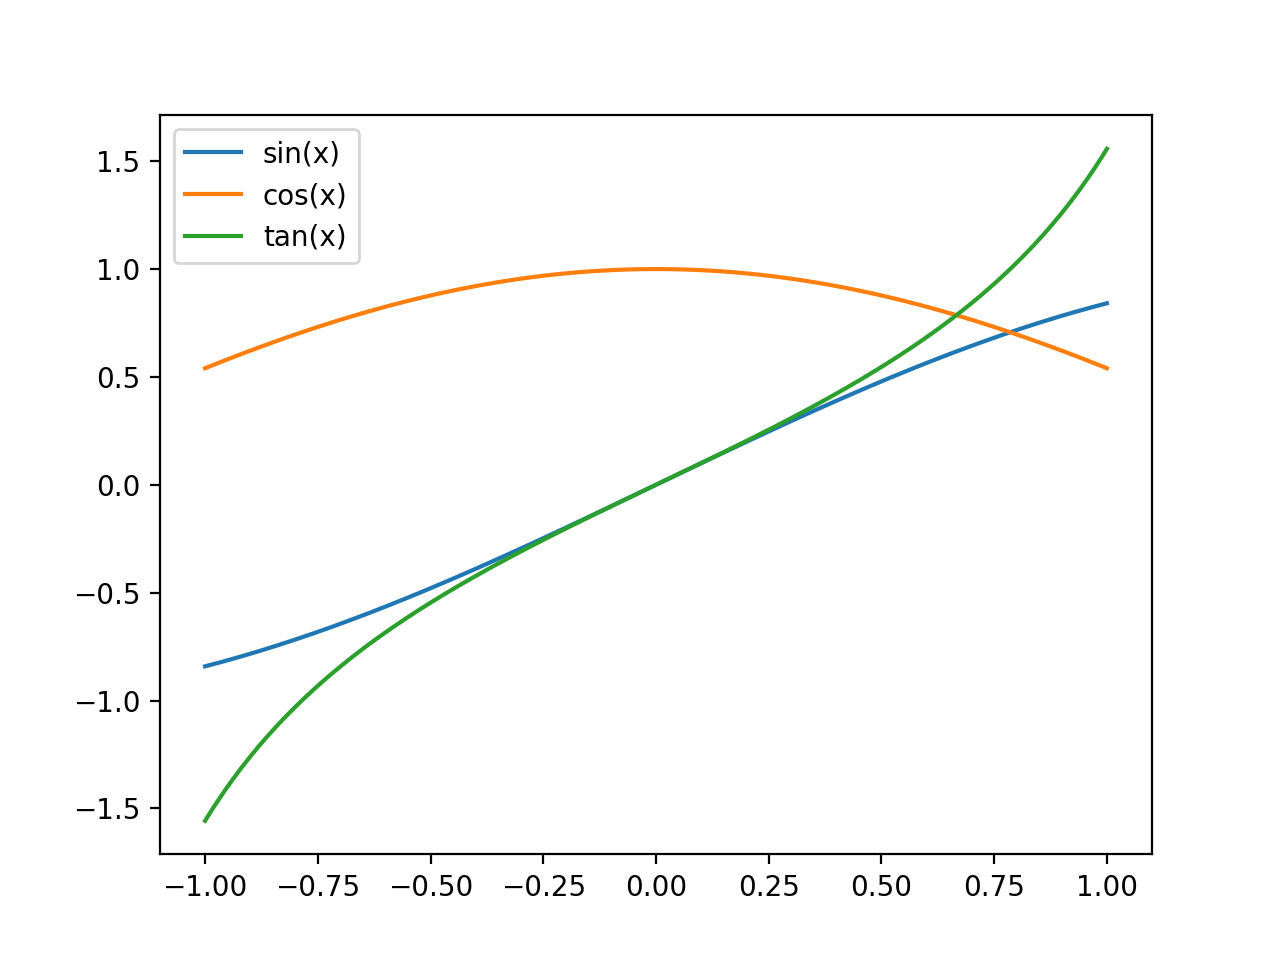
\includegraphics[width=0.5\textwidth]{legend.png}
\end{figure}

If we like to have no frame for the legend bar we can use the command \te{plt.legend(frameon=False)}.
\lstinputlisting[language=Python]{legendframeless.py}
\begin{figure}[h]\centering
\caption{Frameless Legend}
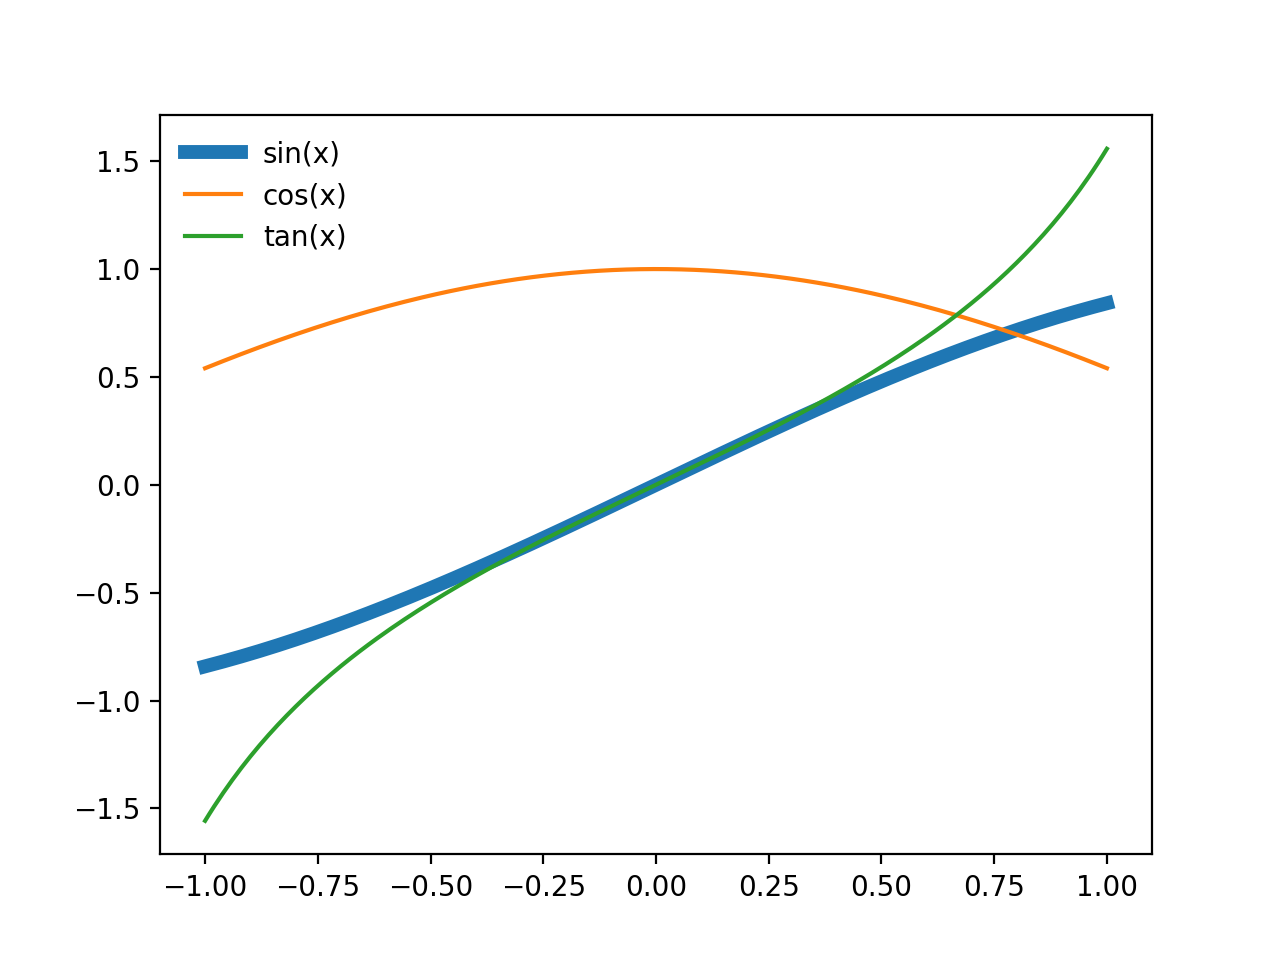
\includegraphics[width=0.5\textwidth]{legendframeless.png}
\end{figure}

Matplotlib is not the only package for data visualisation in python. For further information, you might take a look at \href{http://ggplot.yhathq.com/how-it-works.html}{ggplot} package.


\subsection{Colors}
There are several ways to pick colours for a plot. There are some default colours that we can use right away. They are: [`blue', `green', `red', `cyan', `magenta', `yellow', `black',`white'], and they are referred as  [`b', `g', `r', `c', `m', `y', `k',`w']. One other option is to use the \te{xkcd} package. These are 954 most common RGB monitor colours. To see the list of colours available see for instance \href{https://xkcd.com/color/rgb/}{here}. 

Another option is to specify the colour using RGB code. In the RGB code, the colours Red, Green and Blue are specified each on a scale between black and white. Matplotlib allows to specify their brightness between 0 and 1, or between 0 and 255 in the hexadecimal system \footnote{for instance: `\#48a7f9' corresponds to (48, a7, f9)=($4\times 16^1+8\times 16^0, 10\times 16^1+7\times 16^0, 15\times 16^1+9\times 16^0$)=(72, 167, 249). }.
Option 1: color=(0.5,1.0,0.0)
Option 2: color=`\#48a7f9'
\lstinputlisting[language=Python]{all_colour.py}
\begin{figure}[h]\centering
\caption{Colours}
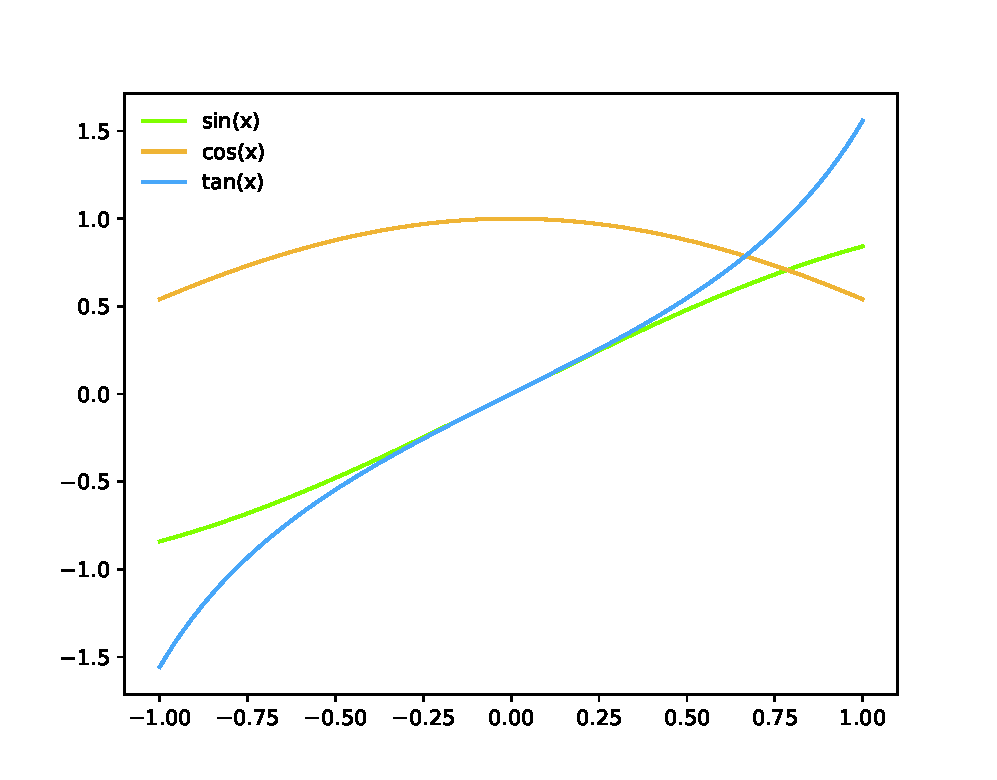
\includegraphics[width=0.5\textwidth]{all_colour.pdf}
\end{figure}




\subsection{Margins}
If we want to make the frame fit to the data, then we can use the command \te{plt.margins(0)}. This is the example of the legend \ref{legend}.
\lstinputlisting[language=Python]{margin.py}

\begin{figure}[h]\centering
\caption{Margin}
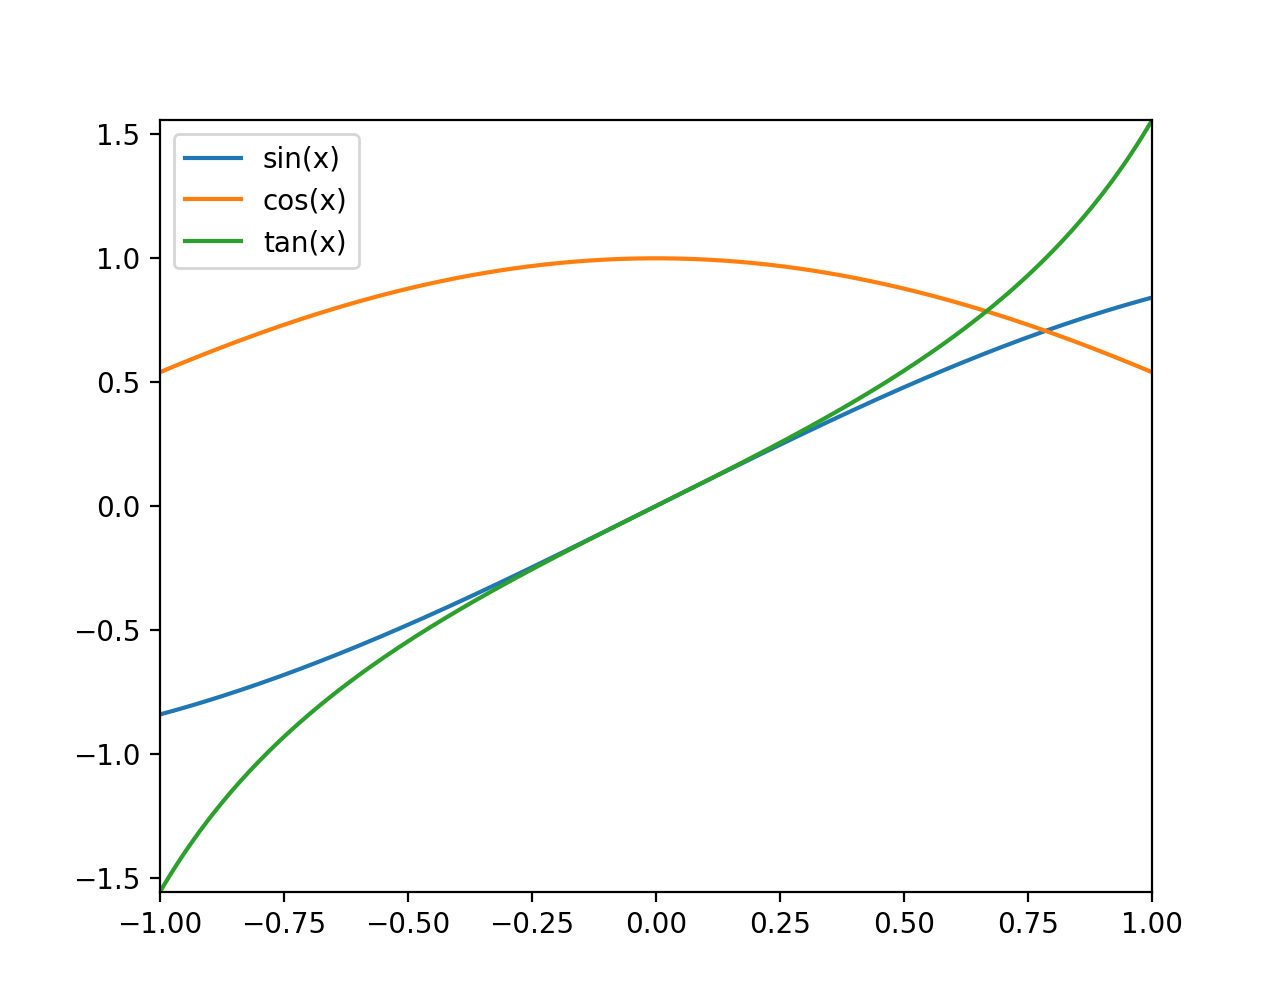
\includegraphics[width=0.5\textwidth]{margin.png}
\end{figure}

The parameter given to the \te{plt.margin} function tells the size of the margin between the extreme points (the left-most, right-most, lowest and highest points) and the border of the plot. The value is relative to the distance between opposite extreme points. That means: If our data starts at the x-position of 0 and ends at the x-position of 2.5, then margin parameter of 1 would lead to the plot starting at $x_{min}-margin_x*(x_{max}-x_{min}) = -2.5$ and ending at $x_{max}-margin_x*(x_{max}-x_{min}) = 5$. The same principle applies for the y-axis. The function can be called with one parameter that applies to both the x- and y-axis, or with two parameters that may differ for x- and y-axis.
Example:


\lstinputlisting[language=Python]{margin1.py}

\begin{figure}[h]\centering
\caption{Margin}
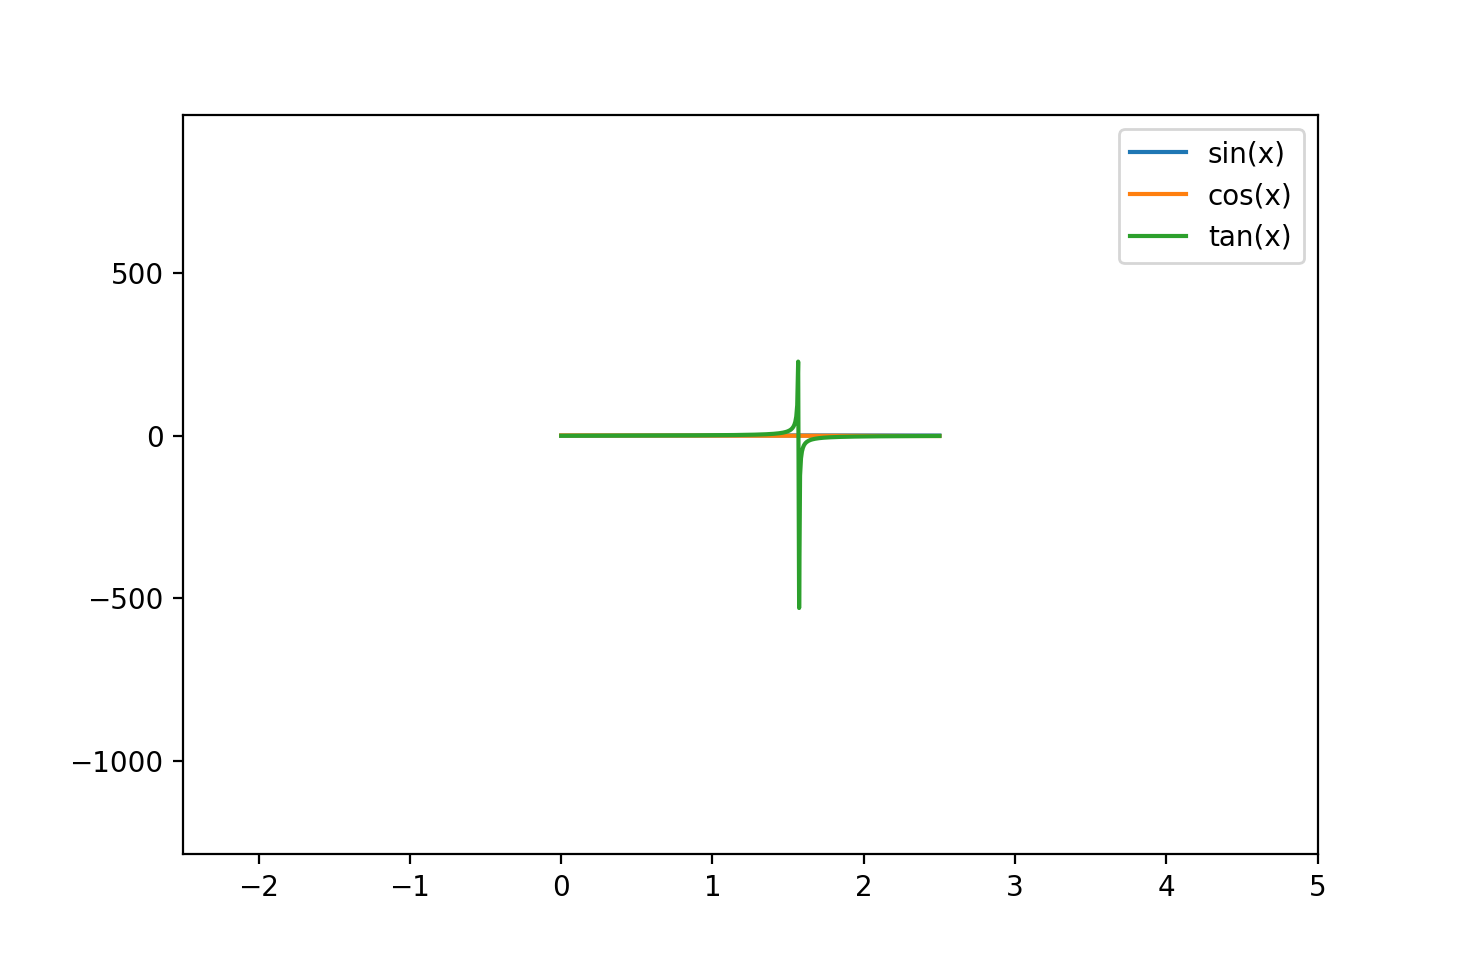
\includegraphics[width=0.5\textwidth]{margin1.png}
\end{figure}








%%%%%%%%%%%%%%%%%%%%%%%%%%%%%%%%%%%%% PANDAS %%%%%%%%%%%%%%%%%%%%%%%%%%%%%%%%%%%%%%%%


\section{Pandas} \label{pandas}
Pandas is a high level data manipulation tool. Pandas has two notable data structure \footnote{some data type that stores data in structured way, for example a NumPy array}, the data frame and series. Unlike NumPy array, Pandas data frames can hold data of different types. Here  we give an example to read the data from a file and store it in a pandas data frame. Here is the data for coronavirus report of 2020-05-15 of some countries. 
\lstinputlisting[]{2020-05-15_Corona_Cases.csv}
and here is the code for reading the data with pandas.
\lstinputlisting[language=Python]{corona_cases.py}
As you noticed the row labels, the country codes that we want to use as row indices, are seen  seen as a column in their own right. To solve this, we use \te{index\_col=0}. This will make the zeroth column to be considered as the indexing column. Alternatively one can set the name of the column as string. 
\lstinputlisting[language=Python]{corona_cases_2.py}

\subsection{Selection}
One of the powerful thing that we can do with pandas is accessing the column easily. Here is an example, we use the previous example, and we want to get the column for \te{Cases}. Alternatively, We can also use the dot notation: \te{data.Recovered}

\lstinputlisting[language=Python]{pandas_select.py}

This way we get a pandas series. If we want to select multiple columns we need to use pandas dataframe structure, example follows
\lstinputlisting[language=Python]{pandas_multiple_select.py}

To access the row we need to use \te{loc} in the way described here.
\lstinputlisting[language=Python]{row_pandas.py}
To access one value you can use \te{loc} again as follows. 
\lstinputlisting[language=Python]{element_pandas.py}
\subsubsection{Conditional Selection}
In order to figure out the index of a row, we can select it by a condition. The following example can illustrate that. There we want to know the \te{Trieste} province row index. To do so we need to look up in the column which has the name of the provinces.
\lstinputlisting[language=Python]{find_trieste.py}

\subsection{Column manipulation}
We can also add a column as well as adding a column based on the other columns. Here is an example:
\lstinputlisting[language=Python]{pandas_column.py}
Since pandas is based on numpy, you can treat column and rows as a numpy array and we can apply arithmetic operations on them.





















%%%%%%%%%%%%%%%%%%%%%%%%%%%%%%%%%%%%% SCIKIT-LEARN %%%%%%%%%%%%%%%%%%%%%%%%%%%%%%%%%%%%%%%%

\section{Scikit-Learn}
Machine Learning is the study of algorithms that improve their estimate of structures in data by learning from data. It includes three major branches:
\begin{itemize}
\item Supervised Learning, solving the task of classification or regression
\item Unsupervised Learning, solving the task of clustering
\item Reinforcement Learning, solving a step-wise optimisation task
\end{itemize}
There are also sub-branches and hybrid approaches such as Semi-Supervised Learning or Self-Supervised Learning.

Scikit-Learn is a python library that implements important steps in the machine learning workflow. This includes not only the machine learning algorithms themselves, but also other important steps, such as the preprocessing of the data.



\subsection{Supervised Learning}
In supervised learning the machine tries to learn patterns from the given data.

Let's imagine we are the machine and we want to learn from a simple dataset.
For that let's consider some data from the weather forecast. Note that this example is to simplify the concept of supervised learning and has nothing to do with reality.
We are given data for temperature and wind speed for three consecutive days. Temperature and wind speed are the \textit{attributes} of the day. Each day belongs to one of two \textit{classes}: Rain or no rain. So we get one data point for each day. We call these data points \textit{instances}.


% Please add the following required packages to your document preamble:
% \usepackage{longtable}
% Note: It may be necessary to compile the document several times to get a multi-page table to line up properly
\begin{longtable}{|l|l|l|l|}
\hline
Day & Temperature & Wind speed & Rain \\ \hline

 Monday& 20 &5&Yes  \\ \hline
Tuesday & 25 & 4 &No\\ \hline
Wednesday &27  & 3&? \\ \hline
\end{longtable}
We want to know whether it will rain on Wednesday. One idea is that we find the most similar day and predict based on that. To find out the closest case to Wednesday is to simply find out the distance in sort of a vector space, where temperature is one axis and wind is another axis.
Therefore we have
\begin{align}\nonumber
D(Wed-Tue)=\sqrt{(27-25)^2+(3-4)^2)}=\sqrt{5}=2.2\\
D(Wed-Mon)=\sqrt{(27-20)^2+(3-5)^2)}=\sqrt{53}=7.3
\end{align}
As you see the closest condition to Wednesday is on Tuesday. Therefore, just a naive prediction is that on Wednesday it might not rain. We assume a class boundary passing in the middle between the instances, where everything on one side belongs to one class and everything on the other side belongs to the other. Such a class boundary is called a \textit{concept}. More generally, a concept is a function which maps instances to classes that they are a member of. 

This form of classification where you consider the nearest instances in the vector space is called ``k-nearest-neighbours"-classifier, or ``kNN" for short. $k$ is a parameter that tells how many nearest neighbours the algorithm should look at. What we have described is a 1-NN (for 1-nearest-neighbour) classifier, so it only looks at the single nearest neighbouring data point. It is also possible to look at, for example, the 15 nearest data points and predict the class that most of the 15 neighbours belong to. This would be a 15-NN classifier.

We assume that there is a function that tells the relation between attributes and the class, but we don't know this function. A supervised learning algorithm tries to induct this function from examples, where it knows the attributes and the corresponding class. Induction means to find general rules from examples. After it has inducted the function, it can deduct the classes of new data points from that function.

The most easy example that we can think of is the daily sunrise: We have seen that the sun rose today, and yesterday, and the day before, and the day before that. From those samples, we \textit{induct} that it rises every day. This is a general rule inducted from sample observations. From there, we can \textit{deduct} whether the sun will rise again tomorrow - we will predict that it will rise.

Let us have a closer look at Supervised Learning. A simple example consists of three steps:
\begin{itemize}
\item Splitting the data into training and test sets
\item Fitting the classifier to the data
\item Evaluating the quality of the classifier for the data we are dealing with
\end{itemize}

\subsubsection{kNN in Scikit-Learn}
Scikit-learn has implemented the kNN classifier. In order to see how well the kNN classifier classifies the data, we would make an experiment. We take the  data in which we already know  their appropriate classes. We then split the data into two different distinct sets. One called training, and the other called testing. In general the fraction of the data which goes to the training part is larger than the testing. In the training part, we give both the data for attribute space and their classes to the machine. We aim to teach the machine how attribute space is associated to their classes. In the testing part, we try to see if the machine actually learnt enough from the training part. We give the data of attribute values of the testing set, but not their classes. Then we ask the machine to predict their classes. As we already know their appropriate classes, we can find out how close the prediction was with their actual class. This way, we can learn how much our kNN classifier is reliable. In the following code we first split the data into training and test set, then make the classifier learn on the training set, and then compare the prediction of the classifier on the test set with the actual classes in the test set. We used example data  which was generated in a supervised learning approach for finding appropriate behaviour of robot swarms. (swarm behaviour) 
\lstinputlisting[language=Python]{classifier.py}\label{classifier.py}


\subsection{Limitations of supervised learning}
In general, the more data we have the more reliable the prediction becomes. However, there are a few issues with both the data and the classifier that can cause the learning to underperform. We mention some of them in the following.
\subsubsection{Insufficient coverage of the attribute space} \label{insuf}
It is important that the data contains samples for most of the attribute space. For example, if the classifier has never seen a day with more than 35 degrees and more than 75 km/h wind speed, then it cannot learn whether it is more likely to rain or not on such a day. If it needs to classify such a day, it may well not be accurate, even if it has seen a lot of colder or less windy days. %There are also other conditions that may lead to unreliable predictions. Some of them are as follows.
\subsubsection{Biased Data}\label{biased}
In the process of training the machine, there might be some occasion that the machine gets biased based on the data given. For example, let's consider the case where a satellite takes a lot of photos from giraffes in savanna and train the machine that they belongs to them. However, it turns out that machine couldn't distinguish them later on. The problem was that the photos that previously shown to machine as giraffe were taken in a cloudy day. The machine has identified giraffes by the weather not the features of the giraffes. When they took other photos of the giraffes in a sunny day, machine was not able to recognise them well. We call this kind of issues as biased data.

Let's give another example for biased data: Assume we have only the body height of people and we want to predict whether the people are men or women. Our training data might be biased if, for example, the men happened to be Japanese and the women South Sudanese, or if the men were measured in the evening (when people are smaller) and the women in the morning. In those cases, the bias is probably big enough to completely distort our predictions, so that they do not generalize to people from different countries, or to measurements taken over the course of the day.
\subsubsection{Lack of Information}\label{lack}
The data might not contain the information that is necessary to predict the class. For example, the relation from temperature and wind to rainfall is weak. Imagine there are many days where the temperature is 20 degrees and the wind speed is 5 km/h and it rained, and many others where the temperature and wind speed are the same, but it did not rain. If this is the case, then the classifier cannot achieve good accuracy of prediction, because the data does not contain enough information. Rain does not only depend on temperature and wind speed, but also on the level of clouds, on relative humidity, on air pressure, on records of rain in surrounding areas, etc. All of this information is missing in our data, so the classifier cannot be accurate. 

%comparison
Just as a comparison among  these three limitations, i.e insufficient coverage of the attribute space, biased data, and lack of information, we give extra explanation as follows. Let's explain the insufficient coverage of the attribute space  \ref{insuf} with another  simple weather forecast scenario; in general if the wind is more than 200 km/h, it rains. However, we only give training  data of wind which is just below 100 km/h.  If we  ask the machine to classify whether it rains if the wind is  215 km/h, then the machine simply cannot predict this. This kind of limitation is related to the distribution of the attributes. As a comparison, if we have a lack of information (\ref{lack}), the problem is about the class. Let's say we have multiple days where the wind was "exactly" 30 km/h. In some of them it rained, in others not. This means that from the wind speed alone, we cannot decide whether it will rain or not, at least not surely. We need other attributes in connection with the wind, so we can make more reliable predictions. A case of biased data would be if, in general, it rains when the wind is strong, and it doesn't rain when the wind is weak, but for some reason, we happen to have measured the exceptions to this rule for our training data. For example, we took all the measurements of strong winds in the desert, and all the measurements of weak wind in the rain-forest. If a classifier gets such data only, it will learn that strong winds lead to dry weather and weak winds to rain. So the problem with biased data is an untypical relation between the attributes and the classes in the training data, which is not representative of the actual concept to be learned.
\subsubsection{Lack of Complexity of the classifier (``underfitting")}
The data might contain the necessary information, but the relation between the attributes and the class might be complex. For example, a simple relation would be that if the temperature is below 25 degrees, then it rains. A complex relation would be that it rains if and only if the temperature is between 19 and 21 degrees and the wind speed is between 5 and 8 km/h, or if the temperature is between 23 and 25 degrees and the wind speed is not between 2 and 4 km/h, and so on. We know all the information that we need to predict whether it rains or not.
Imagine you draw a diagram with temperature on the x-axis and wind-speed on the y-axis, and mark the area where it rains. We say, the class ``rain" occupies a certain area in the configuration space (spanned by temperature and wind-speed). In this case, there are three unconnected areas where it rains: One between 19 and 21 degrees and between 5 and 8 km/h. One between 23 and 25 degrees and between 0 and 2 km/h. And finally, one between 23 and 25 degrees and wind-speed above 4 km/h.
%\todo{But the classifier might not be able to learn this,\\ because it is multimodal}

Some simple classifiers are unable to identify multiple unconnected regions of the same class in the configuration space. They are only able to draw one line that is supposed to separate the two classes (in case of a two-class-problem). Such classifiers are therefore not complex enough to perform well on our complex weather problem. We say, they are underfitting the data. It means that the decision boundary that the classifier draws and that is supposed to separate the classes is not taking the data into account sufficiently to provide good results.

\subsubsection{Over-complexity of the classifier (``overfitting")}
Data conveys a general relationship between attributes and classes. However, the individual data points are often subject to noise, or the classes have some overlap. In our example of the weather forecast, perhaps the measurement equipment has occasional error, or there are certain weather conditions where both rain and not rain is possible. An easier example is when we try to find out whether a person is a man or a woman by only knowing their body height. The body heights are normally distributed. The distributions have, of course, some overlap. That means, if a person is 1.95m, it is more likely to be a man than a woman, but there are occasionally women of that height.  A classifier could over-adapt to the data it has seen (we call this ``overfitting the data"). If, for example, due to randomness, there is a woman of height 1.95 and there is no man of that exact height, then an overfitting classifier would predict any person of that height to be a woman. Since in the height range around 1.95 there are more men, so a meaningful classifier should generalize and learn that within that range, a person is more likely to be a man.

\subsection{Imbalanced Classes}
Let us come back to our example where we want to classify whether a person is a man or a woman based on their height. If we have a sample of the general population in our training set, we would reach some accuracy. It might classify a person with 1.65m as a woman. However, there might be occasions where the classes are not equally distributed. Let us assume we collect (in random order) the height of a group where there are a lot more men than women (such as the Iranian Parliament). There, for example, we have only 16 women and over 200 men (2020). While the women might be smaller than the men on average, using a knn would probably still predict any height to be a man. This is because there are so many more men than women, that even at heights of a typical woman, there will be more men with that height (because height is normally distributed). This issue becomes worse with higher values of k, because there are not enough data points of women to gain the majority at any point in the attribute space.
%TODO: Learn how to make a comment. Write why we need to split the data into training and testing sets.

\subsection{Why splitting the data is important}
In our example code \ref{classifier.py}, we split the data into two sets before learning: training and test (or validation). This is very important to detect overfitting. The classifier learns from the training data (we say it "fits the training data"). After learning, we use the test dataset in order to find out how well it learned. We should not do that only on the training dataset, because the classifier might have overfitted to the training data. If a classifier performs well on the training data, but poor on the test data, it means it has over-adapted to the training data and not learned generally enough to also classify data of the same distribution properly.

\subsubsection{Cross Validation}
We have previously seen that we need to split the data into training and test sets. For parameter optimization (see section \ref{subsubsec:find_best_k}), we also need a validation set. This means that a large part of our data is not available for training. And on the other hand, the test and validation sets might also be small if we have a limited number of data points.
To resolve this, we use a technique called cross-validation. It reuses the same data for several training and testing runs. At first, we split the data into a number of folds (10 in our example). Then, for each training run, we use 9 of those folds for training and 1 for validation. In the first run, for example, we use the first fold as validation and all others as training. In the second run, we use the second fold as validation and all others as training, and so on.
Resulting from this, we get as many accuracy values as we have folds. In order to estimate which parameter setting has the best overall accuracy, we can take the mean or median.
If we have a lot of data, then it does not matter which data points are in the training and test sets, because any particularities average out due to the high number of data points. In any case, it makes sense to shuffle the data beforehand to avoid order bias. The train-test-split function does that automatically.
\subsubsection{Finding the best parameter setting (k) using cross validation}
\label{subsubsec:find_best_k}
We have understood how kNN works, but we don't know how to choose k. We have to try it out for the dataset at hand. In order to try it out, it is not enough to split the data into training and testing, because the best value for k on the testing set might have overadapted to the specific testing set.
In the following code, we use Cross-Validation to find the best value for k.
\lstinputlisting[language=Python]{classification_with_scikit_learn.py}\label{classification_with_scikit_learn.py}

\subsection{Unsupervised Learning}
Another major branch of machine learning does not involve class labels. Instead, it searches for connections of attributes, patterns and correlations in the data. For instance, considering the previous example of weather forecast, in the unsupervised learning, machine would try to collect the data points in groups that have similar temperatures and wind speeds. It organises them in sets of similar properties. This technique is called clustering. However, there are other techniques that use unsupervised learning such as Encoding and Feature Analysis.
They all have a common point that there is no ground truth given. Unsupervised learning can help to find the approximate function in the supervised learning process.

\subsubsection{Encoding}
\subsubsection{Feature Analysis}
\subsection{Reinforcement Learning}
In Reinforcement learning problems, the computer makes multiple decisions before being told how good the decisions were. It only knows how good that combination of decisions was, not individual decisions. The task is to make better decisions on the next try. It is therefore necessary that it has multiple attempts to improve its understanding of which decisions are good. For example, in a new game that the computer doesn't know, it would not know whether any of its moves were good or bad until someone tells it that it won or lost the game. It can only learn which decisions were good or bad by playing the game again, making different decisions, and again wait for the outcome.

%%%%%%%%%%%%%%%%%%%%%%%%%%%%%%%%%%%%%SCIPY %%%%%%%%%%%%%%%%%%%%%%%%%%%%%%%%%%%%%%%%




\section{SciPy}

SciPy is the collections of scientific packages, which is applicable for data analysis. It uses NumPy, but has more feature.
















%%%%%%%%%%%%%%%%%%%%%%%%%%%%%%%%%%%%%YT-TOOLKIT %%%%%%%%%%%%%%%%%%%%%%%%%%%%%%%%%%%%%%%%




\section{yt-toolkit}






















%%%%%%%%%%%%%%%%%%%%%%%%%%%%%%%%%%%%% DICTIONARY%%%%%%%%%%%%%%%%%%%%%%%%%%%%%%%%%%%%%%%%




\section{Glossary}


\subsection{Enumerate}
\label{enumerate}
This is a built-in function in python which counts or get the indices  of items.
\lstinputlisting[language=Python]{enumerate.py}


\subsection{Init function}
\label{subsec:init}
here is an example of init function:
\lstinputlisting[language=Python]{init.py}
you can alternatively have the following code which does the same job:
\lstinputlisting[language=Python]{noinit.py}


\subsection{Main condition} \label{main}
Sometimes we want to run certain codes to test some functions or classes or else in the file, however, we prefer when we import the file which contains the code to some other files that test function doesn't run again. In this case we use the main condition. In the following you can see an example of two files the first one is the file which contains the main condition, and the other on is the file that call the first file to use the class which is defined in the first file.
\lstinputlisting[language=Python]{main_file.py}
the following is the second file where we import the class Person into it, considering that it does not print the test functions.
\lstinputlisting[language=Python]{main_example.py}


\subsection{Range} \label{range}
we can use range function to generate a sequence of numbers, similar to \ref{arange}. There are three ways to do so.
\begin{enumerate}
\item given a number
\item given starting and ending number
\item given starting and ending number with defined step
\end{enumerate}
here is the example
\lstinputlisting[language=Python]{range.py}
\subsection{ravel()}
It is a function to flatten the data.
\lstinputlisting[language=Python]{ravel.py}
Another example:
\lstinputlisting[language=Python]{ravel2.py}


\subsection{Basic Git}
It is often important to work in a code with other people. However, working together sometimes cause conflicts. As changes of someone might not be compatible with the changes of the other person. \te{Git} is a version control system that facilitate group working. Git is particularly suitable for raw text files not for compiled files. Git repository is also useful to store data in a machine readable form.  To learn more about it you may check \href{https://www.atlassian.com/git/tutorials}{this link}.
In order to use git command from within a python script, we need to have a package called \te{git python} installed. 
First if your operating system doesn't have \te{git} installed already by default, you need to install \te{git} first. Find out how to install it \href{https://git-scm.com/}{here}.
After that to install \te{git python} you can use the following command:
\te{pip3 install gitpython}. In order to use it in a code you need to \te{import git}. The documentation of gitpython can be found \href{https://gitpython.readthedocs.io/en/stable/intro.html}{here}.













%%%%%%%%%%%%%%%%%%%%%%%%%%%%%%%%%%%%% EXERCISE %%%%%%%%%%%%%%%%%%%%%%%%%%%%%%%%%%%%%%%%



\section{Exercise}


\begin{enumerate}
\item Write a code that computes the mean value of a given numpy array. %1
\item Write a code that takes the number of participants who want to make a  ping pong tournament and generates a simple match among them. This requires to make a random matching among participants and makes rounds of winners. You may use the knock-out algorithm for simplicity.  %2
\item Write a code that takes the data of COVID-19 from a github resource, for example \href{https://github.com/pcm-dpc/COVID-19/tree/master/dati-province}{here}. Plot the daily new cases for a chosen city, like: Trieste, as well as daily new cases.
\end{enumerate}

\section{Answer}
\begin{enumerate}
\item An answer: \\  %2
\lstinputlisting[language=Python]{mean.py}
\item A sample answer: \\
\lstinputlisting[language=Python]{match.py}
\item A proposed answer (this answer has been manipulated slightly by removing the peculiar negative values for the daily new cases reported  as to represent the data in aesthetic way)
\lstinputlisting[language=Python]{daily_cases_trieste.py}

\begin{figure}[h]\centering

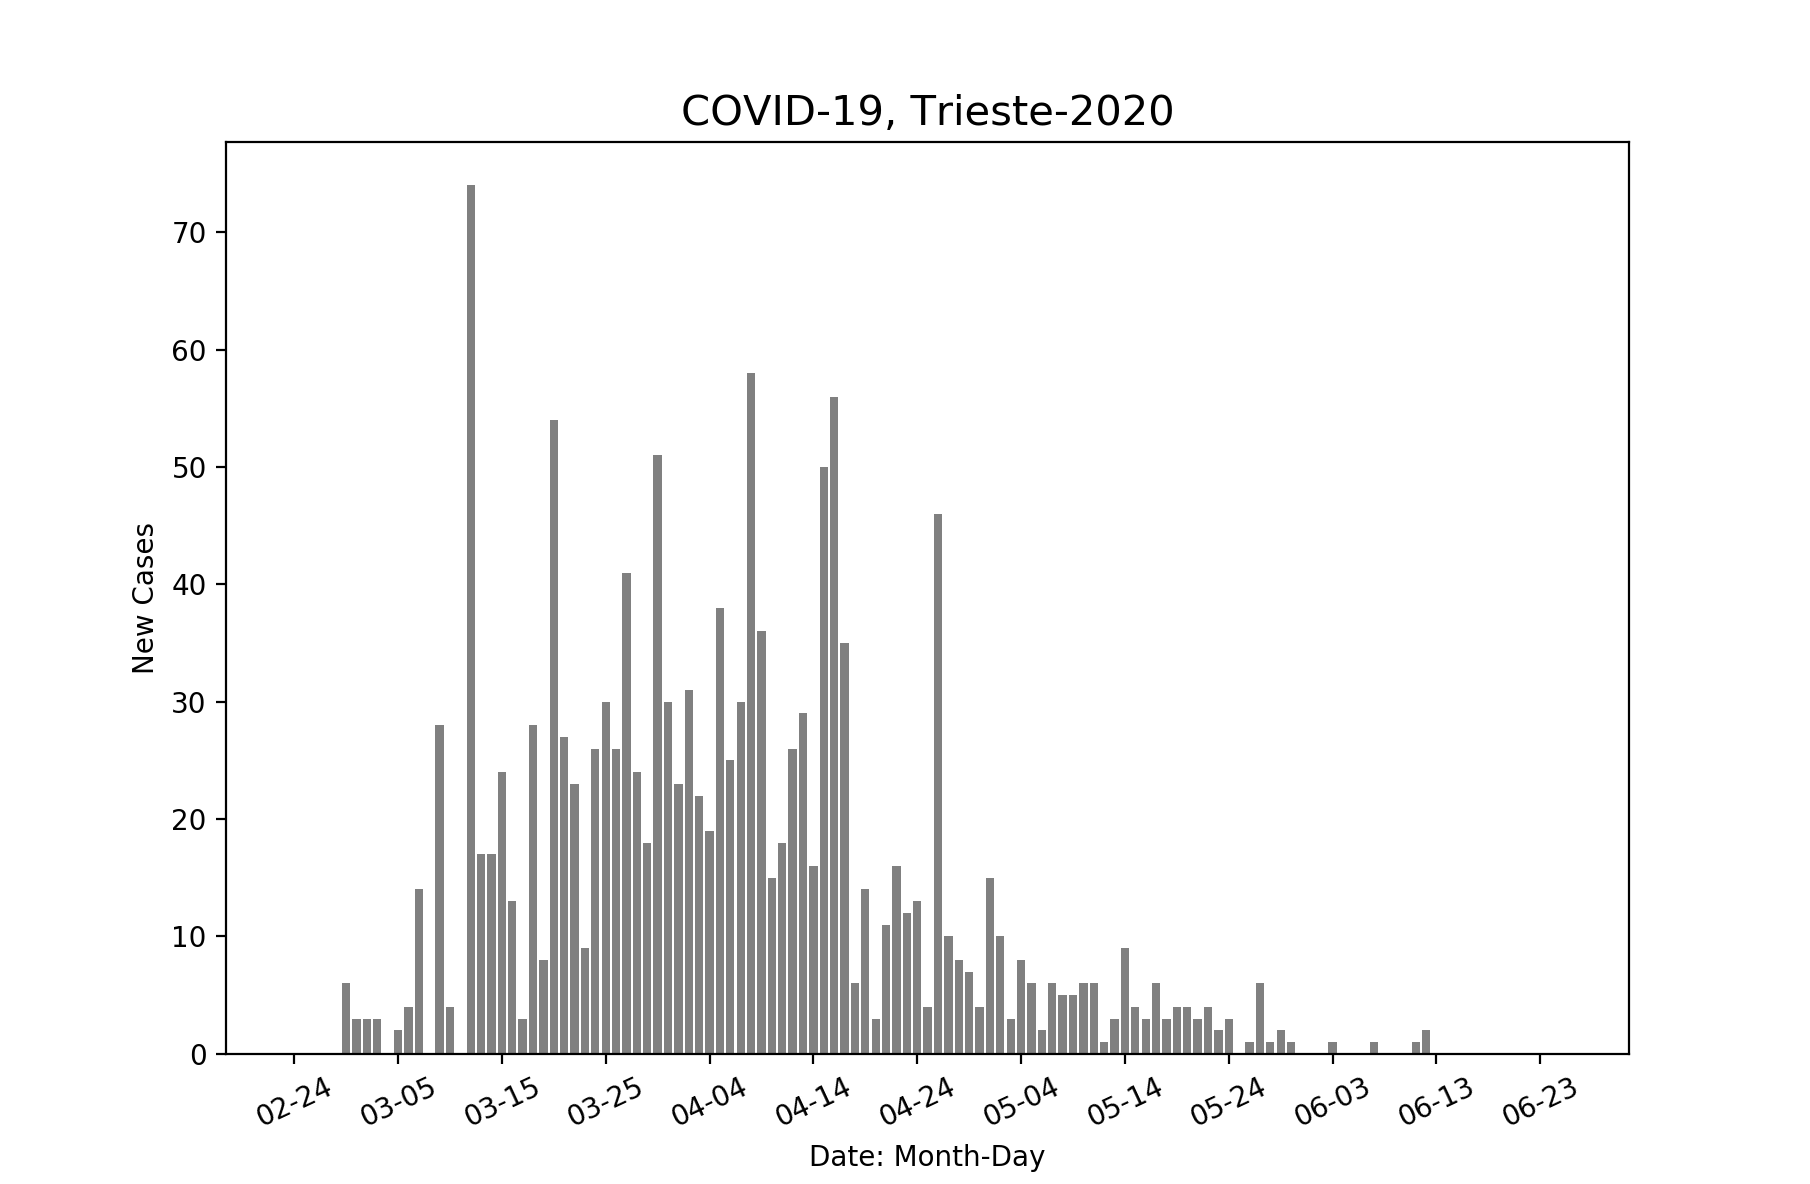
\includegraphics[width=1.0\textwidth]{daily_cases_trieste.png}
\end{figure}

\end{enumerate}






\bibliographystyle{plain}
\bibliography{refe}
\end{document}\lstinputlisting[language=Python]{Classification_With_Scikit-Learn.ipynb}\label{Classification With Scikit-Learn.ipynb}

